
\documentclass[
    12pt,       % Tamanho da fonte
    oneside,    % para impressão apenas no recto. Oposto a twoside
    a4paper,	% Tamanho do papel
    english,    % idioma adicional para hifenização
    french,		% idioma adicional para hifenização
	spanish,	% idioma adicional para hifenização
    brazil      % O último idioma é o principal do documento
    ]{abntex2}

%% ---
% Pacotes fundamentais 
% ---
\usepackage[utf8]{inputenc} % Codificação do documento (conversão automática dos acentos)
\usepackage[T1]{fontenc}    % Seleção de códigos de fonte
\usepackage{pslatex}		% Fonte parecida com a Times New
\usepackage{lmodern}        % Usa a fonte Latin Modern
\usepackage{cmap}	        % Mapear caracteres especiais no PDF
\usepackage{amsmath,amssymb,amsfonts,textcomp} % Fontes matemáticas
\usepackage{graphicx}       % Inclusão de gráficos
\usepackage{color}          % Controle das cores
\usepackage{microtype}      % Para melhorias de justificação
\usepackage{indentfirst}    % Indenta o primeiro parágrafo de cada seção.
\usepackage{nomencl}        % Lista de símbolos
\usepackage[algoruled,algochapter,longend,portuguese]{algorithm2e}	% Permite incluir algoritmos no PDF
\usepackage{makecell}       %
\usepackage{pdfpages}
\usepackage{fancyvrb}

\usepackage{caption}
\usepackage{subcaption}

\usepackage{appendix}
\usepackage{listings}       %Inserir códigos
\usepackage{xcolor}

%Setando as características dos códigos

\definecolor{codegreen}{rgb}{0,0.6,0}
\definecolor{codegray}{rgb}{0.5,0.5,0.5}
\definecolor{codepurple}{rgb}{0.58,0,0.82}
\definecolor{backcolour}{rgb}{0.95,0.95,0.92}

\lstdefinestyle{mystyle}{
    backgroundcolor=\color{backcolour},   
    commentstyle=\color{codegreen},
    keywordstyle=\color{magenta},
    numberstyle=\tiny\color{codegray},
    stringstyle=\color{codepurple},
    basicstyle=\ttfamily\footnotesize,
    breakatwhitespace=false,         
    breaklines=true,                 
    captionpos=t,                    
    keepspaces=true,                 
    numbers=left,                    
    numbersep=5pt,                  
    showspaces=false,                
    showstringspaces=false,
    showtabs=false,                  
    tabsize=2
}

\lstset{style=mystyle}
% ---

% ---
% Pacotes adicionais, usados apenas no âmbito do Modelo Canônico do abnteX2
% ---
\usepackage{lipsum}				% para geração de dummy text
% ---

% ---
% Pacotes de citações
% ---
\usepackage[brazilian,hyperpageref]{backref}    % Paginas com as citações na bibl
\usepackage[alf]{abntex2cite}	                % Citações padrão ABNT
% ---
%% --- 
% CONFIGURAÇÕES
% --- 

% ---
% Reestrutura a fonte do capítulo e da sessão
% ---
\renewcommand{\ABNTEXchapterfont}{\fontseries{b}}
\renewcommand{\ABNTEXchapterfontsize}{\large}
\renewcommand{\ABNTEXsectionfont}{\fontseries{m}}
\renewcommand{\ABNTEXsectionfontsize}{\normalsize}
\renewcommand{\ABNTEXsubsectionfont}{\fontseries{b}}
\renewcommand{\ABNTEXsubsectionfontsize}{\normalsize}
\renewcommand{\ABNTEXsubsubsectionfont}{\fontseries{m}}
\renewcommand{\ABNTEXsubsubsectionfontsize}{\normalsize}
% ---

% ---
% Configurações do pacote backref
% Usado sem a opção hyperpageref de backref
\renewcommand{\backrefpagesname}{Citado na(s) página(s):~}
% Texto padrão antes do número das páginas
\renewcommand{\backref}{}
% Define os textos da citação
\renewcommand*{\backrefalt}[4]{
	\ifcase #1 %
		Nenhuma citação no texto.%
	\or
		Citado na página #2.%
	\else
		Citado #1 vezes nas páginas #2.%
	\fi}%
% ---

% ---
% Informações de dados para CAPA e FOLHA DE ROSTO
% ---
\instituicao {
Instituto Federal da Paraíba\\
Coordenação de Pós-graduação em Engenharia Elétrica\\
Disciplina: Processamento Digital de Imagens
}

\titulo {Relatório\\Atividade Avaliativa da Aula 3}

\tipotrabalho {Relatório}

\autor {Nayana Priscylla Nery dos Santos \\
        Jônatas Mendes da Cruz \\
        Sérgio Ricardo Maciel Pedrosa}
\orientador {Carlos Danilo Miranda Régis, Dr.}
\coorientador{}

\local {João Pessoa - PB}
\date {Setembro de 2023}

\preambulo{\textbf{Relatório apresentado ao professor Carlos Danilo Miranda Régis, referente a atividade avaliativa da terceira aula da disciplina de Processamento Digital de Imagens, do Programa de Pós-Graduação em Engenharia Elétrica do Instituto Federal de Educação, Ciência e Tecnologia da Paraíba}}
% ---

% ---
% Folha da capa
% ---
\renewcommand{\imprimircapa}
{
  \begin{capa}
    \begin{center}
        
\includegraphics[width=15.5cm,keepaspectratio]{Elementos/Figuras/Figuras capa/header.jpg}
        \large\imprimirinstituicao
        \vspace{5cm}

       	\large\imprimirautor
    
        \vspace*{\fill}
       		\large\imprimirtitulo
        \vspace*{\fill}
        
        \normalsize\imprimirlocal
        \par
        \normalsize\imprimirdata
    \end{center}
  \end{capa}
}
% ---

% ---
% Folha de rosto
% ---
\renewcommand{\imprimirfolhaderosto}
{
    \begin{folhaderosto}
        \begin{center}
            Instituto Federal da Paraíba\\
            Programa de Pós-graduação em Engenharia Elétrica\\
            Disciplina: Ferramentas para Análise e Processamento de Sinais\\

            \imprimirautor

            \vspace*{\fill}
            {\large\imprimirtitulo}
            \vspace*{\fill}
        
            \hspace{.45\textwidth}
            \begin{minipage}
                {.5\textwidth}
                \imprimirpreambulo
            \end{minipage}
               
            \vspace*{\fill}
       	    \textbf{Orientador:} \large\imprimirorientador
            \vspace*{\fill}
        
            \normalsize\imprimirlocal
            \par
            \normalsize\imprimirdata
        \end{center}
    \end{folhaderosto}
}
% ---

% ---
% Altera as margens padrões
% ---
\setlrmarginsandblock{3cm}{2cm}{*}
\setulmarginsandblock{3cm}{2cm}{*}
\checkandfixthelayout
% ---

% --- 
% Espaçamentos entre linhas e parágrafos 
% --- 

% O tamanho do parágrafo é dado por:
\setlength{\parindent}{1.3cm}

% Controle do espaçamento entre um parágrafo e outro:
\setlength{\parskip}{0.2cm}  % tente também \onelineskip

% ---
% compila o índice
% ---
\makeindex
% ---
% ---
% Pacotes fundamentais 
% ---
\usepackage[utf8]{inputenc} % Codificação do documento (conversão automática dos acentos)
\usepackage[T1]{fontenc}    % Seleção de códigos de fonte
\usepackage{pslatex}		% Fonte parecida com a Times New
\usepackage{lmodern}        % Usa a fonte Latin Modern
\usepackage{cmap}	        % Mapear caracteres especiais no PDF
\usepackage{amsmath,amssymb,amsfonts,textcomp} % Fontes matemáticas
\usepackage{graphicx}       % Inclusão de gráficos
\usepackage{color}          % Controle das cores
\usepackage{microtype}      % Para melhorias de justificação
\usepackage{indentfirst}    % Indenta o primeiro parágrafo de cada seção.
\usepackage{nomencl}        % Lista de símbolos
\usepackage[algoruled,algochapter,longend,portuguese]{algorithm2e}	% Permite incluir algoritmos no PDF
\usepackage{makecell}       %
\usepackage{pdfpages}
\usepackage{fancyvrb}

\usepackage{caption}
\usepackage{subcaption}

\usepackage{appendix}
\usepackage{listings}       %Inserir códigos
\usepackage{xcolor}

%Setando as características dos códigos

\definecolor{codegreen}{rgb}{0,0.6,0}
\definecolor{codegray}{rgb}{0.5,0.5,0.5}
\definecolor{codepurple}{rgb}{0.58,0,0.82}
\definecolor{backcolour}{rgb}{0.95,0.95,0.92}

\lstdefinestyle{mystyle}{
    backgroundcolor=\color{backcolour},   
    commentstyle=\color{codegreen},
    keywordstyle=\color{magenta},
    numberstyle=\tiny\color{codegray},
    stringstyle=\color{codepurple},
    basicstyle=\ttfamily\footnotesize,
    breakatwhitespace=false,         
    breaklines=true,                 
    captionpos=t,                    
    keepspaces=true,                 
    numbers=left,                    
    numbersep=5pt,                  
    showspaces=false,                
    showstringspaces=false,
    showtabs=false,                  
    tabsize=2
}

\lstset{style=mystyle}
% ---

% ---
% Pacotes adicionais, usados apenas no âmbito do Modelo Canônico do abnteX2
% ---
\usepackage{lipsum}				% para geração de dummy text
% ---

% ---
% Pacotes de citações
% ---
\usepackage[brazilian,hyperpageref]{backref}    % Paginas com as citações na bibl
\usepackage[alf]{abntex2cite}	                % Citações padrão ABNT
% ---
% --- 
% CONFIGURAÇÕES
% --- 

% ---
% Reestrutura a fonte do capítulo e da sessão
% ---
\renewcommand{\ABNTEXchapterfont}{\fontseries{b}}
\renewcommand{\ABNTEXchapterfontsize}{\large}
\renewcommand{\ABNTEXsectionfont}{\fontseries{m}}
\renewcommand{\ABNTEXsectionfontsize}{\normalsize}
\renewcommand{\ABNTEXsubsectionfont}{\fontseries{b}}
\renewcommand{\ABNTEXsubsectionfontsize}{\normalsize}
\renewcommand{\ABNTEXsubsubsectionfont}{\fontseries{m}}
\renewcommand{\ABNTEXsubsubsectionfontsize}{\normalsize}
% ---

% ---
% Configurações do pacote backref
% Usado sem a opção hyperpageref de backref
\renewcommand{\backrefpagesname}{Citado na(s) página(s):~}
% Texto padrão antes do número das páginas
\renewcommand{\backref}{}
% Define os textos da citação
\renewcommand*{\backrefalt}[4]{
	\ifcase #1 %
		Nenhuma citação no texto.%
	\or
		Citado na página #2.%
	\else
		Citado #1 vezes nas páginas #2.%
	\fi}%
% ---

% ---
% Informações de dados para CAPA e FOLHA DE ROSTO
% ---
\instituicao {
Instituto Federal da Paraíba\\
Coordenação de Pós-graduação em Engenharia Elétrica\\
Disciplina: Processamento Digital de Imagens
}

\titulo {Relatório\\Atividade Avaliativa da Aula 3}

\tipotrabalho {Relatório}

\autor {Nayana Priscylla Nery dos Santos \\
        Jônatas Mendes da Cruz \\
        Sérgio Ricardo Maciel Pedrosa}
\orientador {Carlos Danilo Miranda Régis, Dr.}
\coorientador{}

\local {João Pessoa - PB}
\date {Setembro de 2023}

\preambulo{\textbf{Relatório apresentado ao professor Carlos Danilo Miranda Régis, referente a atividade avaliativa da terceira aula da disciplina de Processamento Digital de Imagens, do Programa de Pós-Graduação em Engenharia Elétrica do Instituto Federal de Educação, Ciência e Tecnologia da Paraíba}}
% ---

% ---
% Folha da capa
% ---
\renewcommand{\imprimircapa}
{
  \begin{capa}
    \begin{center}
        
\includegraphics[width=15.5cm,keepaspectratio]{Elementos/Figuras/Figuras capa/header.jpg}
        \large\imprimirinstituicao
        \vspace{5cm}

       	\large\imprimirautor
    
        \vspace*{\fill}
       		\large\imprimirtitulo
        \vspace*{\fill}
        
        \normalsize\imprimirlocal
        \par
        \normalsize\imprimirdata
    \end{center}
  \end{capa}
}
% ---

% ---
% Folha de rosto
% ---
\renewcommand{\imprimirfolhaderosto}
{
    \begin{folhaderosto}
        \begin{center}
            Instituto Federal da Paraíba\\
            Programa de Pós-graduação em Engenharia Elétrica\\
            Disciplina: Ferramentas para Análise e Processamento de Sinais\\

            \imprimirautor

            \vspace*{\fill}
            {\large\imprimirtitulo}
            \vspace*{\fill}
        
            \hspace{.45\textwidth}
            \begin{minipage}
                {.5\textwidth}
                \imprimirpreambulo
            \end{minipage}
               
            \vspace*{\fill}
       	    \textbf{Orientador:} \large\imprimirorientador
            \vspace*{\fill}
        
            \normalsize\imprimirlocal
            \par
            \normalsize\imprimirdata
        \end{center}
    \end{folhaderosto}
}
% ---

% ---
% Altera as margens padrões
% ---
\setlrmarginsandblock{3cm}{2cm}{*}
\setulmarginsandblock{3cm}{2cm}{*}
\checkandfixthelayout
% ---

% --- 
% Espaçamentos entre linhas e parágrafos 
% --- 

% O tamanho do parágrafo é dado por:
\setlength{\parindent}{1.3cm}

% Controle do espaçamento entre um parágrafo e outro:
\setlength{\parskip}{0.2cm}  % tente também \onelineskip

% ---
% compila o índice
% ---
\makeindex
% ---

% ----
% Início do documento
% ----
\begin{document}
% % ---
% Pacotes fundamentais 
% ---
\usepackage[utf8]{inputenc} % Codificação do documento (conversão automática dos acentos)
\usepackage[T1]{fontenc}    % Seleção de códigos de fonte
\usepackage{pslatex}		% Fonte parecida com a Times New
\usepackage{lmodern}        % Usa a fonte Latin Modern
\usepackage{cmap}	        % Mapear caracteres especiais no PDF
\usepackage{amsmath,amssymb,amsfonts,textcomp} % Fontes matemáticas
\usepackage{graphicx}       % Inclusão de gráficos
\usepackage{color}          % Controle das cores
\usepackage{microtype}      % Para melhorias de justificação
\usepackage{indentfirst}    % Indenta o primeiro parágrafo de cada seção.
\usepackage{nomencl}        % Lista de símbolos
\usepackage[algoruled,algochapter,longend,portuguese]{algorithm2e}	% Permite incluir algoritmos no PDF
\usepackage{makecell}       %
\usepackage{pdfpages}
\usepackage{fancyvrb}

\usepackage{caption}
\usepackage{subcaption}

\usepackage{appendix}
\usepackage{listings}       %Inserir códigos
\usepackage{xcolor}

%Setando as características dos códigos

\definecolor{codegreen}{rgb}{0,0.6,0}
\definecolor{codegray}{rgb}{0.5,0.5,0.5}
\definecolor{codepurple}{rgb}{0.58,0,0.82}
\definecolor{backcolour}{rgb}{0.95,0.95,0.92}

\lstdefinestyle{mystyle}{
    backgroundcolor=\color{backcolour},   
    commentstyle=\color{codegreen},
    keywordstyle=\color{magenta},
    numberstyle=\tiny\color{codegray},
    stringstyle=\color{codepurple},
    basicstyle=\ttfamily\footnotesize,
    breakatwhitespace=false,         
    breaklines=true,                 
    captionpos=t,                    
    keepspaces=true,                 
    numbers=left,                    
    numbersep=5pt,                  
    showspaces=false,                
    showstringspaces=false,
    showtabs=false,                  
    tabsize=2
}

\lstset{style=mystyle}
% ---

% ---
% Pacotes adicionais, usados apenas no âmbito do Modelo Canônico do abnteX2
% ---
\usepackage{lipsum}				% para geração de dummy text
% ---

% ---
% Pacotes de citações
% ---
\usepackage[brazilian,hyperpageref]{backref}    % Paginas com as citações na bibl
\usepackage[alf]{abntex2cite}	                % Citações padrão ABNT
% ---
% % --- 
% CONFIGURAÇÕES
% --- 

% ---
% Reestrutura a fonte do capítulo e da sessão
% ---
\renewcommand{\ABNTEXchapterfont}{\fontseries{b}}
\renewcommand{\ABNTEXchapterfontsize}{\large}
\renewcommand{\ABNTEXsectionfont}{\fontseries{m}}
\renewcommand{\ABNTEXsectionfontsize}{\normalsize}
\renewcommand{\ABNTEXsubsectionfont}{\fontseries{b}}
\renewcommand{\ABNTEXsubsectionfontsize}{\normalsize}
\renewcommand{\ABNTEXsubsubsectionfont}{\fontseries{m}}
\renewcommand{\ABNTEXsubsubsectionfontsize}{\normalsize}
% ---

% ---
% Configurações do pacote backref
% Usado sem a opção hyperpageref de backref
\renewcommand{\backrefpagesname}{Citado na(s) página(s):~}
% Texto padrão antes do número das páginas
\renewcommand{\backref}{}
% Define os textos da citação
\renewcommand*{\backrefalt}[4]{
	\ifcase #1 %
		Nenhuma citação no texto.%
	\or
		Citado na página #2.%
	\else
		Citado #1 vezes nas páginas #2.%
	\fi}%
% ---

% ---
% Informações de dados para CAPA e FOLHA DE ROSTO
% ---
\instituicao {
Instituto Federal da Paraíba\\
Coordenação de Pós-graduação em Engenharia Elétrica\\
Disciplina: Processamento Digital de Imagens
}

\titulo {Relatório\\Atividade Avaliativa da Aula 3}

\tipotrabalho {Relatório}

\autor {Nayana Priscylla Nery dos Santos \\
        Jônatas Mendes da Cruz \\
        Sérgio Ricardo Maciel Pedrosa}
\orientador {Carlos Danilo Miranda Régis, Dr.}
\coorientador{}

\local {João Pessoa - PB}
\date {Setembro de 2023}

\preambulo{\textbf{Relatório apresentado ao professor Carlos Danilo Miranda Régis, referente a atividade avaliativa da terceira aula da disciplina de Processamento Digital de Imagens, do Programa de Pós-Graduação em Engenharia Elétrica do Instituto Federal de Educação, Ciência e Tecnologia da Paraíba}}
% ---

% ---
% Folha da capa
% ---
\renewcommand{\imprimircapa}
{
  \begin{capa}
    \begin{center}
        
\includegraphics[width=15.5cm,keepaspectratio]{Elementos/Figuras/Figuras capa/header.jpg}
        \large\imprimirinstituicao
        \vspace{5cm}

       	\large\imprimirautor
    
        \vspace*{\fill}
       		\large\imprimirtitulo
        \vspace*{\fill}
        
        \normalsize\imprimirlocal
        \par
        \normalsize\imprimirdata
    \end{center}
  \end{capa}
}
% ---

% ---
% Folha de rosto
% ---
\renewcommand{\imprimirfolhaderosto}
{
    \begin{folhaderosto}
        \begin{center}
            Instituto Federal da Paraíba\\
            Programa de Pós-graduação em Engenharia Elétrica\\
            Disciplina: Ferramentas para Análise e Processamento de Sinais\\

            \imprimirautor

            \vspace*{\fill}
            {\large\imprimirtitulo}
            \vspace*{\fill}
        
            \hspace{.45\textwidth}
            \begin{minipage}
                {.5\textwidth}
                \imprimirpreambulo
            \end{minipage}
               
            \vspace*{\fill}
       	    \textbf{Orientador:} \large\imprimirorientador
            \vspace*{\fill}
        
            \normalsize\imprimirlocal
            \par
            \normalsize\imprimirdata
        \end{center}
    \end{folhaderosto}
}
% ---

% ---
% Altera as margens padrões
% ---
\setlrmarginsandblock{3cm}{2cm}{*}
\setulmarginsandblock{3cm}{2cm}{*}
\checkandfixthelayout
% ---

% --- 
% Espaçamentos entre linhas e parágrafos 
% --- 

% O tamanho do parágrafo é dado por:
\setlength{\parindent}{1.3cm}

% Controle do espaçamento entre um parágrafo e outro:
\setlength{\parskip}{0.2cm}  % tente também \onelineskip

% ---
% compila o índice
% ---
\makeindex
% ---
% Seleciona o idioma do documento (conforme pacotes do babel)
\selectlanguage{brazil}

% Retira espaço extra obsoleto entre as frases.
\frenchspacing 

% ---
% Capa
% ---
\imprimircapa
% ---
% ---

% Folha de rosto
% (o * indica que haverá a ficha bibliográfica)
% ---
\imprimirfolhaderosto
% ---
% ---
% inserir lista de ilustrações
% ---
\pdfbookmark[0]{\listfigurename}{lof}
\listoffigures*
\cleardoublepage
% ---

% ---
% inserir lista de tabelas
% ---
\pdfbookmark[0]{\listtablename}{lot}
\listoftables*
\cleardoublepage
% ---

% ---
% inserir lista de abreviaturas e siglas
% ---
% \begin{siglas}
%     \item[IEMD] Image Empirical Mode Decomposition 
%     \item[EMDPL] Empirical Mode Decomposition Phase Locking
%     \item[SNA] Sistema Nervoso Autónomo 
%     \item[MEG] Magnetoencefalografia
%     \item[Hz] Hertz
%     \item[TF] Transformada de Fourier
%     \item[IMF] Intrinsic Mode Function
%     \item[EMD] Empirical Mode Decomposition
%     \item[HSA] Analise Espectral de Hilbert
%     \item[HHT] Hilbert-Huang Transform
%     \item[dB] Decibéis
   
    
    
% \end{siglas}
% ---

% ---
% inserir o sumario
% ---
\pdfbookmark[0]{\contentsname}{toc}
\tableofcontents*
\cleardoublepage
% ---

% ---
% ELEMENTOS TEXTUAIS
% ---
\textual
% ---

\chapter[Introdução]{Introdução}

As imagens digitais nem sempre são objetos triviais de se analisar. Muitas vezes, informações importantes podem passar despercebidas e isso pode ocorrer propositalmente ou não. Para resolver esse problema, diferentes técnicas podem ser aplicadas sobre a imagem para que detalhes ocultos venham à tona.

Informações importantes podem ser extraídas por meio da visualização do histograma de uma imagem, e este também pode ser utilizado por algoritmos de filtragem para a aplicação de correções e transformações sobre a imagem alvo. A correção \textit{Gamma} permite que áreas escuras de uma imagem sejam clareadas para que detalhes escondidos possam ser visualizados, e da mesma forma, permite que áreas claras sejam escurecidas, aumentando o destaque das informações ofuscadas pela claridade.

Outra técnica importante é a binarização, que retira todos os detalhes desnecessários de uma imagem, dividindo-a em regiões pretas ou brancas. Algumas vezes, no entanto, o que se deseja não é a visualização de informações ocultas e sim a ocultação de informações em uma imagem. Esse objetivo pode ser alcançado por meio das técnicas de LSB e MSB, dessa forma, informações como textos, imagens ou até áudios podem ser transportadas através de \textit{bits} específicos de cada \textit{pixel} de uma imagem.

A atividade proposta tem como objetivo testar todas as técnicas descritas anteriormente, a fim de demonstrar a sua utilidade para a área de processamento de imagens digitais e visão computacional.


Etapas da atividade:

\begin{enumerate}
    \item Apresentar o Histograma das imagens selecionadas em aulas anteriores;
    \item Clarear e escurecer as imagens (usando dois valores de \textit{gamma}), apresentando também o histograma;
    \item Binarizar as imagens originais e transformadas, por limiar e \textit{Otsu};
    \item \begin{enumerate}
        \item Apresentar as imagens com os \textit{bits} mais e menos significativos;
        \item Substituir com zeros os bits menos significativos e avaliar com as métricas objetivas.
    \end{enumerate}
\end{enumerate}

\chapter[Fundamentação Teórica]{Fundamentação Teórica}

\section{Transformação de Intensidade - Correção \textit{gamma}}

As transformações de intensidade e filtragem espacial cobrem uma ampla variedade de aplicações. Nesta atividade específica a aplicação é o realce de imagens, que é o processo de manipular uma imagem de forma que o resultado seja mais adequado do que o original para um determinado fim.

As transformações de potência apresentam a forma básica \cite{gonzalez2009processamento}:

\begin{equation}\label{eq:gamma}
    s = cr^\gamma
\end{equation}

sendo $c$ e $\gamma$ constantes positivas.

\section{Histograma}

O histograma é um gráfico de distribuição de frequências, onde em uma dimensão desse gráfico estão os valores que se deseja analisar a frequência e em outra estão as frequências desses valores. O histograma de uma imagem digital representa a frequência de cada nível de intensidade que um \textit{pixel} pode ter, sendo que essas frequências são a quantidade ou a porcentagem de \textit{pixels} que possuem determinada intensidade.

\section{Binarização}

A binarização é uma técnica que permite a segmentação de áreas de interesse em uma imagem digital por meio da transformação das tonalidades dos \textit{pixels} da mesma para preto (todos os \textit{bits} são zero) ou branco (todos os \textit{bits} são um).

\subsection{Limiar}

A técnica de binarização utiliza-se de um limiar (\textit{threshold}), que define um ponto de corte para a classificação dos \textit{pixels} de acordo com o seu valor. Os \textit{pixels} que possuem um valor maior do que o limiar tornam-se brancos e os que possuem um valor menor ou igual tornam-se pretos.

\subsection{Otsu}

O método \textit{Otsu} é uma forma de encontrar um limiar de forma dinâmica. Este método utiliza-se do histograma da imagem para encontrar as duas intensidades com maior frequência e a partir delas calcular o melhor limiar para a binarização da imagem. O método de \textit{Otsu} se caracteriza por sua natureza não paramétrica e não supervisionada de seleção de limiar e tem certas vantagens desejáveis, o processo como um todo é muito simples são utilizados somente os momentos cumulativos zero e de primeira ordem do histograma de níveis de cinza; viabilizando a análise de outros aspectos importantes, tais como estimativa dos níveis médios das classes e, separabilidade das classes. Um limiar ótimo (ou conjunto de limiares) é selecionado de forma automática e estável, não baseado na diferenciação (uma propriedade local como um vale) mas sim na integração (propriedade global) do histograma. 

\section{\textit{bits} menos significativos (LSB) e \textit{bits} mais significativos (MSB)}

As imagens digitais são representadas por \textit{pixels}, que nada mais são do que uma sequência de bits que podem ser armazenados e manipulados. Os bits de uma sequência podem ser classificados em dois grupos, os \textit{bits} mais significativos (\textit{Most Significant Bit} – MSB) e os \textit{bits} menos significativos (\textit{Least Significant Bit} – LSB) \cite{Adonias2017}.

Os \textit{bits} menos significativos são aqueles que exercem uma menor influência sobre a informação e que não causam mudanças extremas caso sejam modificados. Os \textit{bits} mais significativos, por sua vez, exercem grande influência sobre a informação e podem causar ruídos muito perceptíveis quando alterados.

\section{\textit{Peak Signal-to-Noise Ratio} (PSNR)}

A PSNR e o \textit{Mean Square Error} (MSE) são métricas comuns na literatura para mensurar a qualidade entre duas imagens. O PSNR indica a semelhança entre duas imagens e é recíproco ao MSE, sendo o PSNR uma representação logarítmica do MSE.

O MSE é calculado a partir do valor médio dos erros quadráticos entre os \textit{pixels} da imagem original e da imagem modificada que está sendo confrontada, sendo definido como:

\begin{equation}\label{eq:psnr1}
    MSE(f,h) = \frac{1}{R . C}\sum_{x=1}^{C}\sum_{y=1}^{R}(f(x,y) - h(x,y))^2,
\end{equation}

onde $R$ é o número total de linhas, $C$ é o número total de colunas e $f(x,y)$ e $h(x,y)$ são os níveis de intensidade de luminância em que $x$ e $y$ representam as coordenadas espaciais de um $pixel$. Quanto melhor a imagem avaliada em relação à original, menor é o valor do MSE \cite{Regis2015}.

A PSNR, medida em decibéis (dB), é inversamente proporcional ao MSE e é definida como

\begin{equation}\label{eq:psnr2}
    PSNR = 10 \cdot {\log_{10} \left[ \frac{{MAX}^2}{MSE(f,h)} \right] } dB,
\end{equation}

em que $MAX = 2^b-1$ é o valor máximo da escala de níveis de cinza construída com $b$ \textit{bits}. Quanto maior o valor da PSNR, maior é a semelhança entre a imagem original e a imagem confrontada.

Sua popularidade se dá devido a facilidade de implementação e rapidez no processamento, porém, a PSNR se baseia em uma comparação \textit{byte} a \textit{byte} dos dados, desconsiderando o que eles realmente representam.


\section{\textit{Structural Similiarity Index} (SSIM)}

O SSIM é uma métrica que utiliza a estatística da imagem para avaliação da qualidade. É construído como um modelo multiplicativo que é constituído de atributos da semelhança estrutural e de informações da luminância e contraste da imagem. 

Sejam dois sinais representados por $f = \{f_i|i = 1, 2, ...,P\}$ e $h = \{h_i|i = 1, 2, ...,P\}$, sendo $f$ a imagem original e $h$ a imagem confrontada, define-se SSIM como

\begin{equation}\label{eq:ssim1}
    SSIM(f,h) = l(f,h)^\alpha \cdot c(f,h)^\beta \cdot s(f,h)^\gamma, 
\end{equation}

em que $l(\cdot)$, $c(\cdot)$ e $s(\cdot)$, indicam luminância, contraste e atributos de semelhança estrutural, respectivamente, e os expoentes $\alpha$, $\beta$ e $\gamma$ são parâmetros utilizados para ajustar a importância de cada atributo e, para efeitos de simplificação, são considerados iguais a $1$.

A luminância mede a intensidade média de cada pixel $(\mu)$ entre $f$ e $h$, e é calculada por

\begin{equation}\label{eq:ssim2}
    l(f,h) = \frac{ 2\mu_f \mu_h + K_1}{\mu_f^2 \mu_h^2 + K_1}
\end{equation}

em que a constante $K_1$ é inserida para evitar instabilidade nos valores como, por exemplo, se o denominador tiver um valor próximo de zero.

Analogamente, a análise do contraste é dada por

\begin{equation}\label{eq:ssim3}
    c(f,h) = \frac{ 2\theta_f \theta_h + K_2}{\theta_f^2 \theta_h^2 + K_2}
\end{equation}

em que o $\theta$ é o desvio padrão.

Por fim, a análise entre as estruturas é dada por

\begin{equation}\label{eq:ssim4}
    s(f,h) = \frac{ 2\theta_{fh} + K_3}{\theta_f + \theta_h + K_3}
\end{equation}

assim como $K_1$, as constantes $K_2$ e $K_3$ são inseridas para evitar instabilidades nos valores.

A técnica SSIM é utilizada para encontrar artefatos em imagens desde que haja outra imagem considerada como referência. Em comparação com a PSNR que estima apenas erros absolutos, o SSIM considera a degradação da imagem como uma alteração na informação estrutural.
\chapter[Metodologia]{Metodologia}
\label{chap:metodologia}

\section{Imagens}
\label{sec:imagens}

Para realização da atividade proposta, foram utilizadas 4 imagens escolhidas aleatoriamente no portal pexels.com, conforme Figura \ref{imagens-rgb}.

\begin{figure}[!htpb]
 \centering
 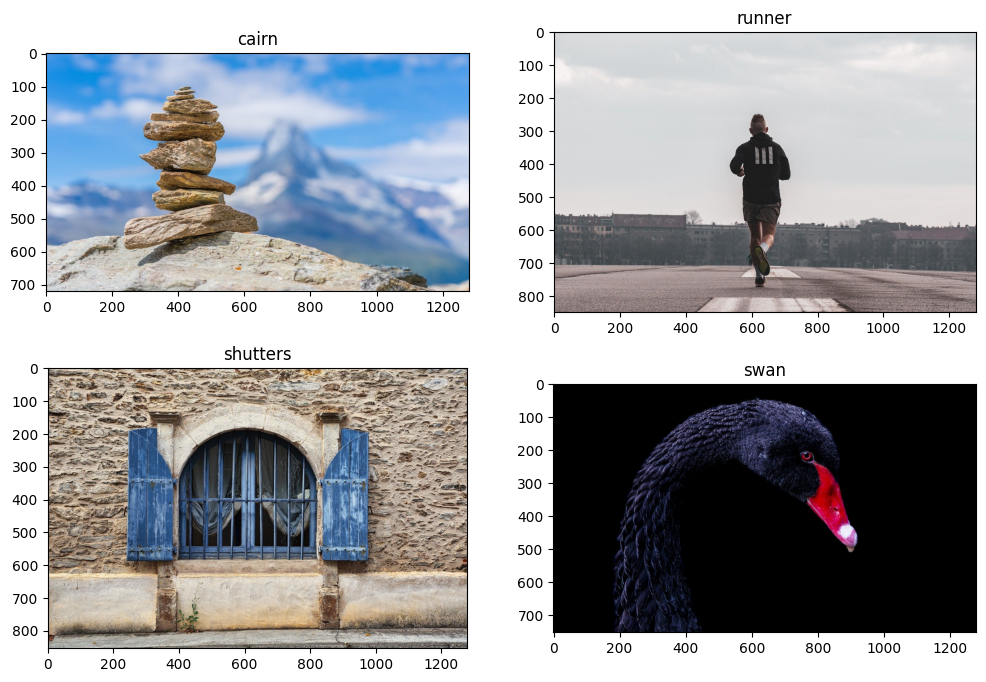
\includegraphics[scale=0.5]{Elementos/Figuras/metodologia-originais-rgb.png}
 \caption{Imagens em RGB}
 \label{imagens-rgb}
\end{figure}

As imagens selecionadas foram pré-processadas e transformadas em escala de cinza, conforme apresentadas na Figura \ref{imagens-gray}, para viabilização das transformações propostas e análise dos resultados obtidos.

\begin{figure}[!htpb]
 \centering
 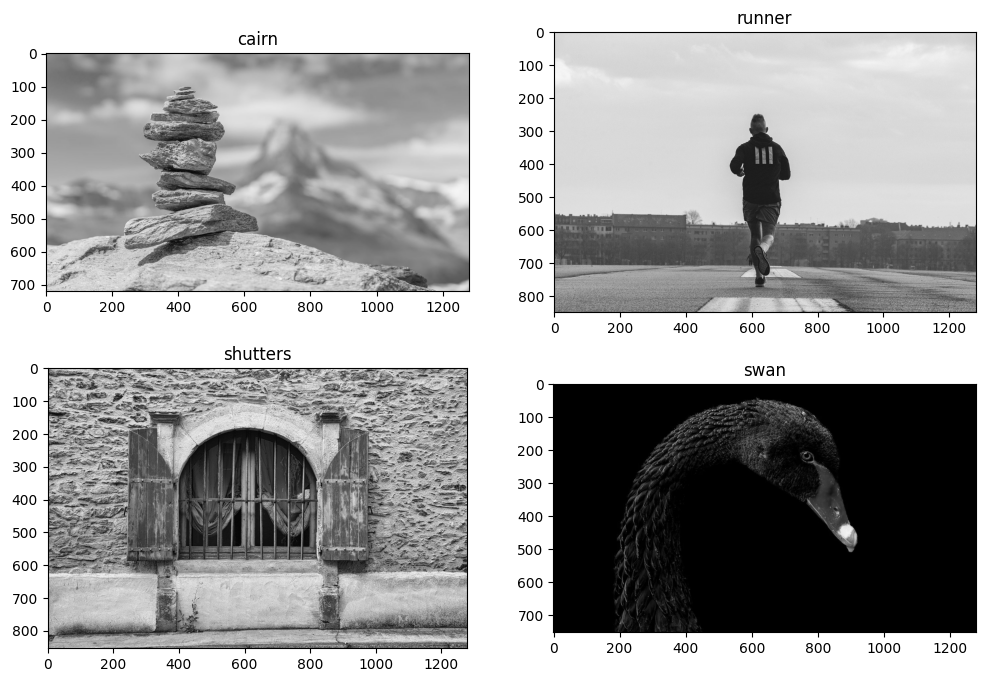
\includegraphics[scale=0.5]{Elementos/Figuras/imagens-originais-gray.png}
 \caption{Imagens em escala de cinza}
 \label{imagens-gray}
\end{figure}

Para um melhor entendimento e interpretação dos resultados, tendo como linha de base as características pertinentes às imagens originais, foram extraídas as informações espaciais das imagens em escala de cinza e exibidas na Figura \ref{imagens-si}: desvio padrão e as imagens resultantes da aplicação do Filtro de \textit{Sobel}.

\begin{figure}[!htpb]
 \centering
 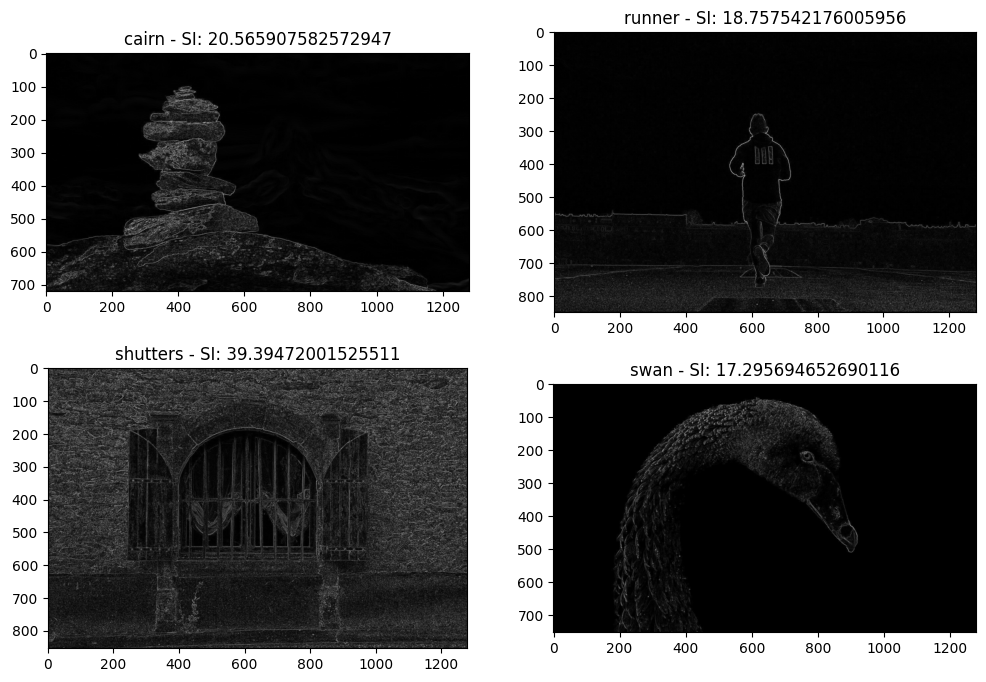
\includegraphics[scale=0.5]{Elementos/Figuras/metodologia-si.png}
 \caption{Imagens resultantes da aplicação do filtro de \textit{Sobel} com as respectivas Informações Espaciais (SI)}
 \label{imagens-si}
\end{figure}

\section{Recursos Computacionais}
\label{sec:recursos}

Para a realização desta atividade avaliativa, foi utilizado o ambiente de desenvolvimento colaborativo \textit{Google Colab} (Figura \ref{imagens-colab}). A linguagem de programação adotada foi \textit{Python} e as bibliotecas especializadas utilizadas neste trabalho de acordo suas aplicações, foram:

\begin{itemize}
    \item \textbf{OpenCV} (cv2) - Manipulação e processamento das imagens;
    \item \textbf{NumPy} (numpy) - Funções matemáticas e operações com vetores e matrizes;
    \item \textbf{scikit-image} (skimage) - Processamento das métricas dos resultados;
    \item \textbf{os} (os) - Interação com o sistema operacional no que tange a manipulação dos arquivos de imagens armazenados no sistema de arquivos;
    \item \textbf{Matplotlib} (matplotlib) - Criação dos gráficos e visualização das imagens e dados.
\end{itemize}


\begin{figure}[!htpb]
 \centering
 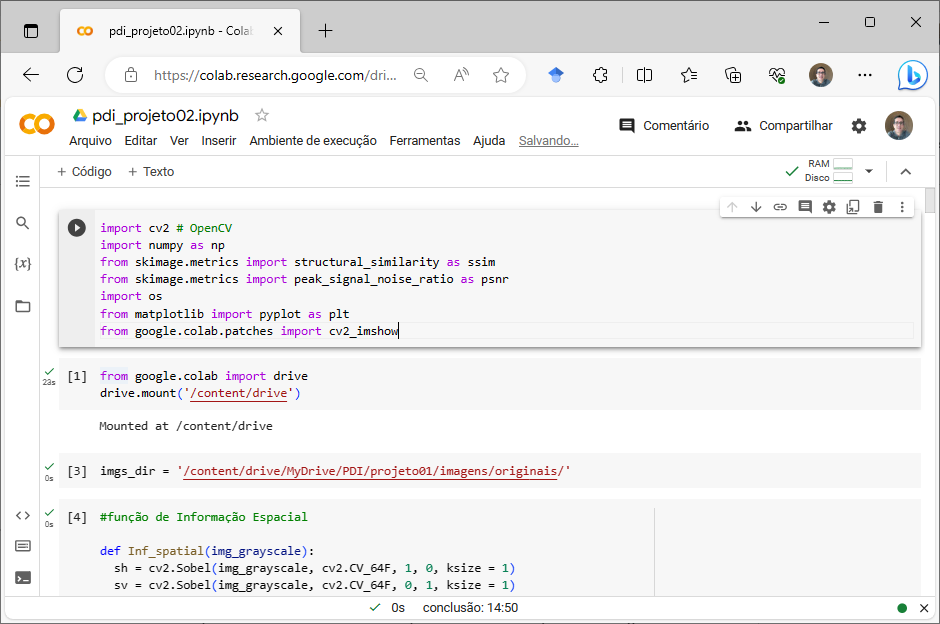
\includegraphics[scale=0.5]{Elementos/Figuras/metodologia-colab.png}
 \caption{Tela do ambiente \textit{Google Colab})}
 \label{imagens-colab}
\end{figure}

% \include{Elementos/4_Experimento}
\chapter[Resultados]{Resultados}

\section{Apresentação dos Histogramas das imagens selecionadas}

Os Histogramas das 4 imagens selecionadas possuem distribuições de valores de \textit{pixels} consideravelmente distintas entre si, como pode ser visualizado nas Figuras \ref{fig:hist-cairn} a \ref{fig:hist-swan}. Destacam-se os Histogramas das imagens \textit{shutters} e \textit{swan}, Figuras \ref{fig:hist-shutters} e  \ref{fig:hist-swan}, respectivamente, por apresentar: a primeira, uma distribuição ao longo de todos valores de \textit{pixels}, sem pico prevalente; a segunda, em oposição àquela, baixa ou nenhuma distribuição, prevalecendo no valor zero, em conformidade com o que é visto na imagem.

\begin{figure}
    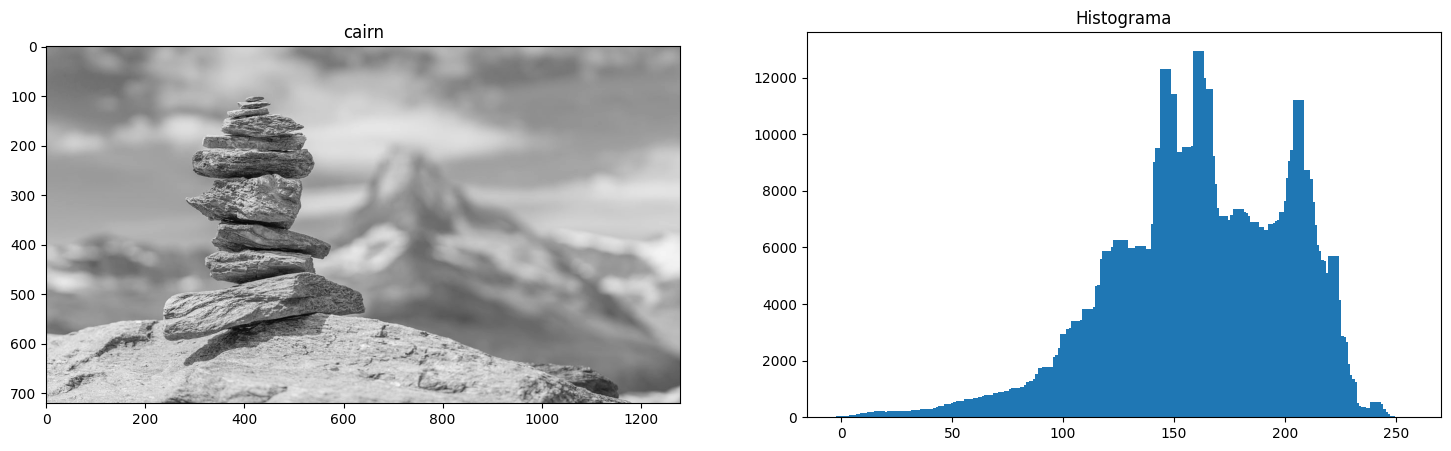
\includegraphics[width=1\linewidth]{Elementos/Figuras/resultados-histograma-cairn.png}
    \caption{Imagem original \textit{cairn} em escala de cinza e o respectivo Histograma}
    \label{fig:hist-cairn}
\end{figure}

\begin{figure}
    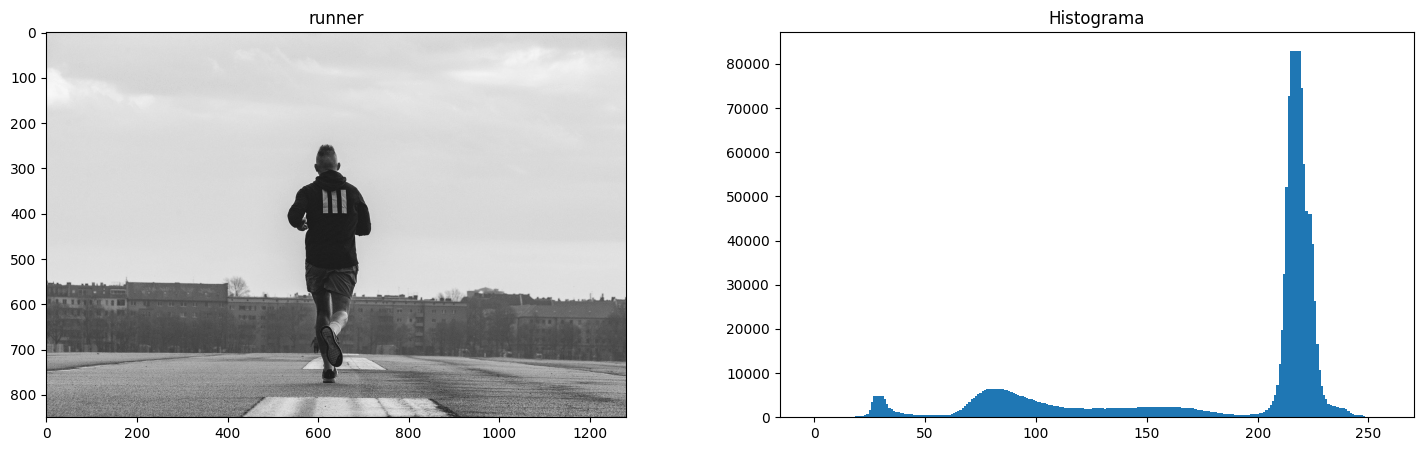
\includegraphics[width=1\linewidth]{Elementos/Figuras/resultados-histograma-runner.png}
    \caption{Imagem original \textit{runner} em escala de cinza e o respectivo Histograma}
    \label{fig:hist-runner}
\end{figure}

\begin{figure}
    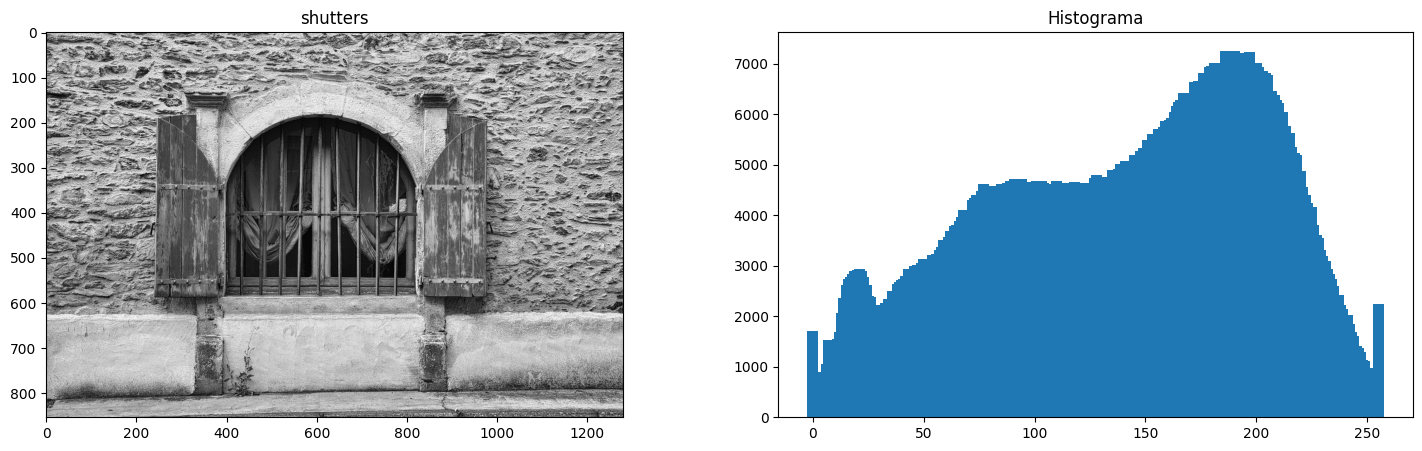
\includegraphics[width=1\linewidth]{Elementos/Figuras/resultados-histograma-shutters.png}
    \caption{Imagem original \textit{shutters} em escala de cinza e o respectivo Histograma}
    \label{fig:hist-shutters}
\end{figure}

\begin{figure}
    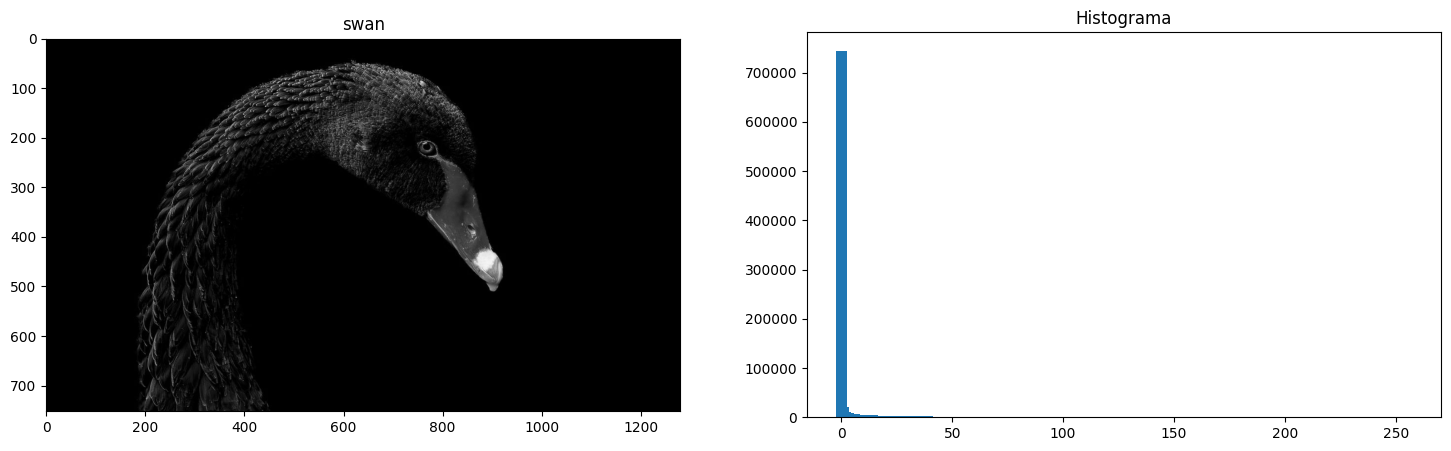
\includegraphics[width=1\linewidth]{Elementos/Figuras/resultados-histograma-swan.png}
    \caption{Imagem original \textit{swan} em escala de cinza e o respectivo Histograma}
    \label{fig:hist-swan}
\end{figure}

% ------------------------------------------------------------- %

\section{Transformação de Intensidade - Correção \textit{gamma}}

Conforme o proposto, foram realizadas duas transformações de intensidade para cada imagem, variando o valor de \textit{gamma} e observados os efeitos que cada aplicação de valor provocou nas imagens. Foram escolhidos: um valor menor que 1 para provocar um deslocamento da distribuição de valores de \textit{pixels} à esquerda, em direção ao zero, resultando em um escurecimento da imagem; e um valor maior que 1 para fazer o deslocamento à direita, em direção ao 255, resultando por conseguinte, em um clareamento da imagem.

As imagens resultantes e seus respectivos Histogramas estão apresentados para visualização e análise nas Figuras \ref{fig:gamma-cairn} a \ref{fig:gamma-swan}. Cada figura contém também a imagem e seu Histograma original para confrontação.

Dos resultados esperados e em conformidade com a transformação realizada, visualiza-se em destaque:

\begin{itemize}
    \item O surgimento de um pico de concentração no escurecimento da imagem \textit{runner} (Figura \ref{fig:gamma-runner});
    \item Na mesma imagem citada no item anterior, no resultado do clareamento, observa-se no Histograma uma separação na distribuição entre os valores de pixel 100 e 150;
    \item Uma forte concentração de valores no escurecimento da imagem \textit{shutters} (Figura \ref{fig:gamma-shutters}), uma vez que originalmente esta imagem possui uma distribuição ao longo de toda a escala de valores;
    \item No escurecimento da imagem \textit{swan} (Figura \ref{fig:gamma-swan}), que originalmente já possui uma concentração predominante em um pico no valor zero, provocou um deslocamento dos poucos valores diferentes de zero, transformando a imagem para quase totalmente zero (preto), fazendo desaparecer a ave objeto da imagem;
    \item Em contrapartida, na mesma imagem citada no item anterior, o clareamento provocou um melhor contorno do objeto da imagem, efeito refletido no respectivo Histograma, através de uma separação observada na distribuição de valores entre os \textit{pixels} de intensidade zero e aproximadamente 30.
\end{itemize}


\begin{figure}
    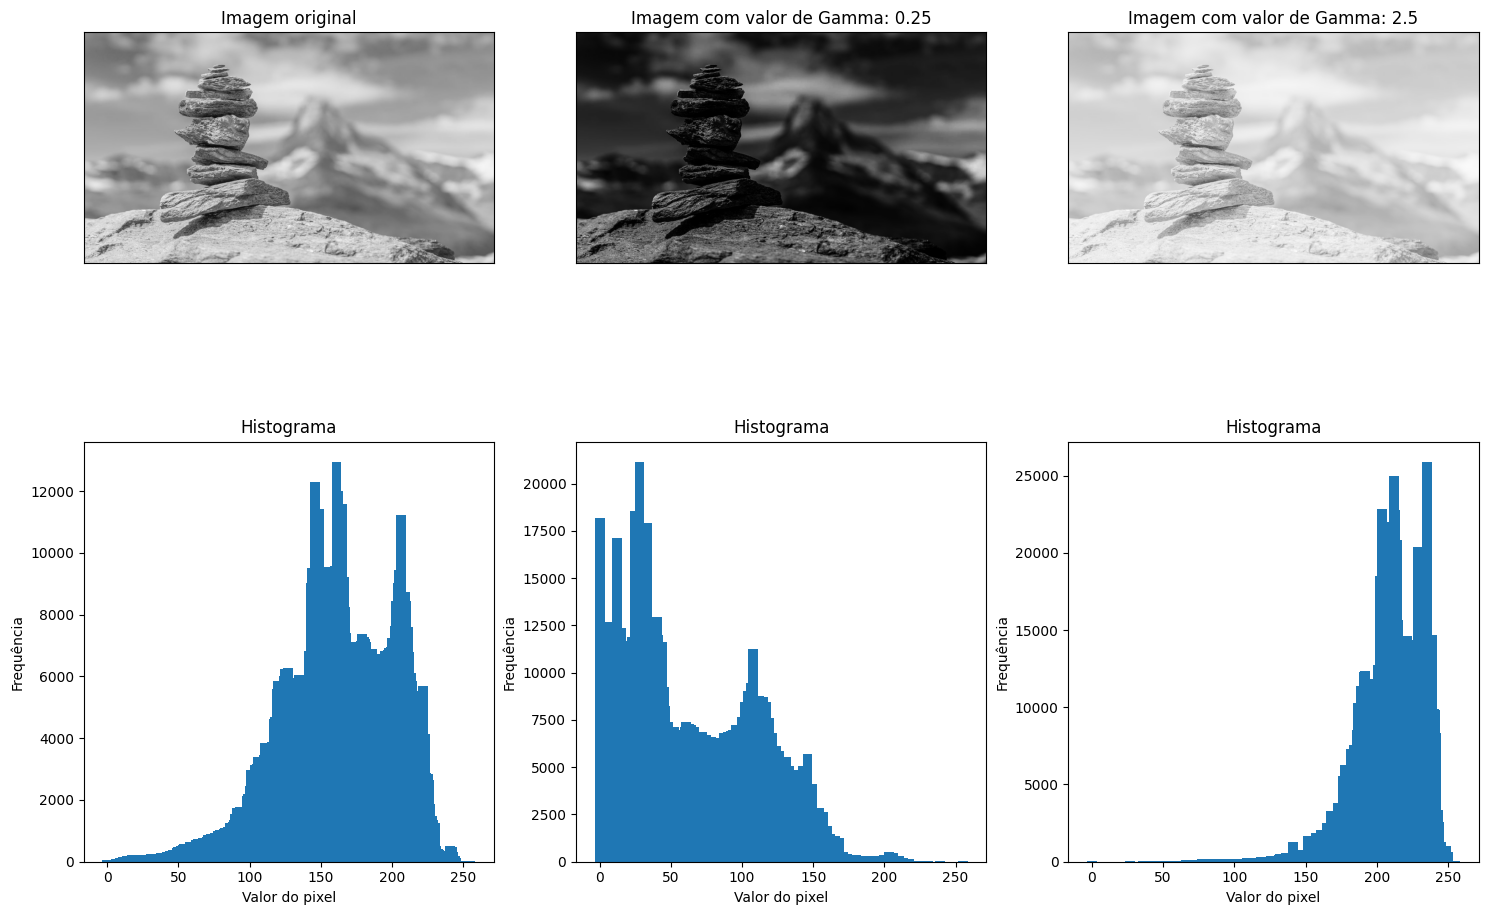
\includegraphics[width=1\linewidth]{Elementos/Figuras/resultados-gamma-cairn.png}
    \caption{Imagem \textit{cairn} em transformação por \textit{Gamma Correction}}
    \label{fig:gamma-cairn}
\end{figure}

\begin{figure}
    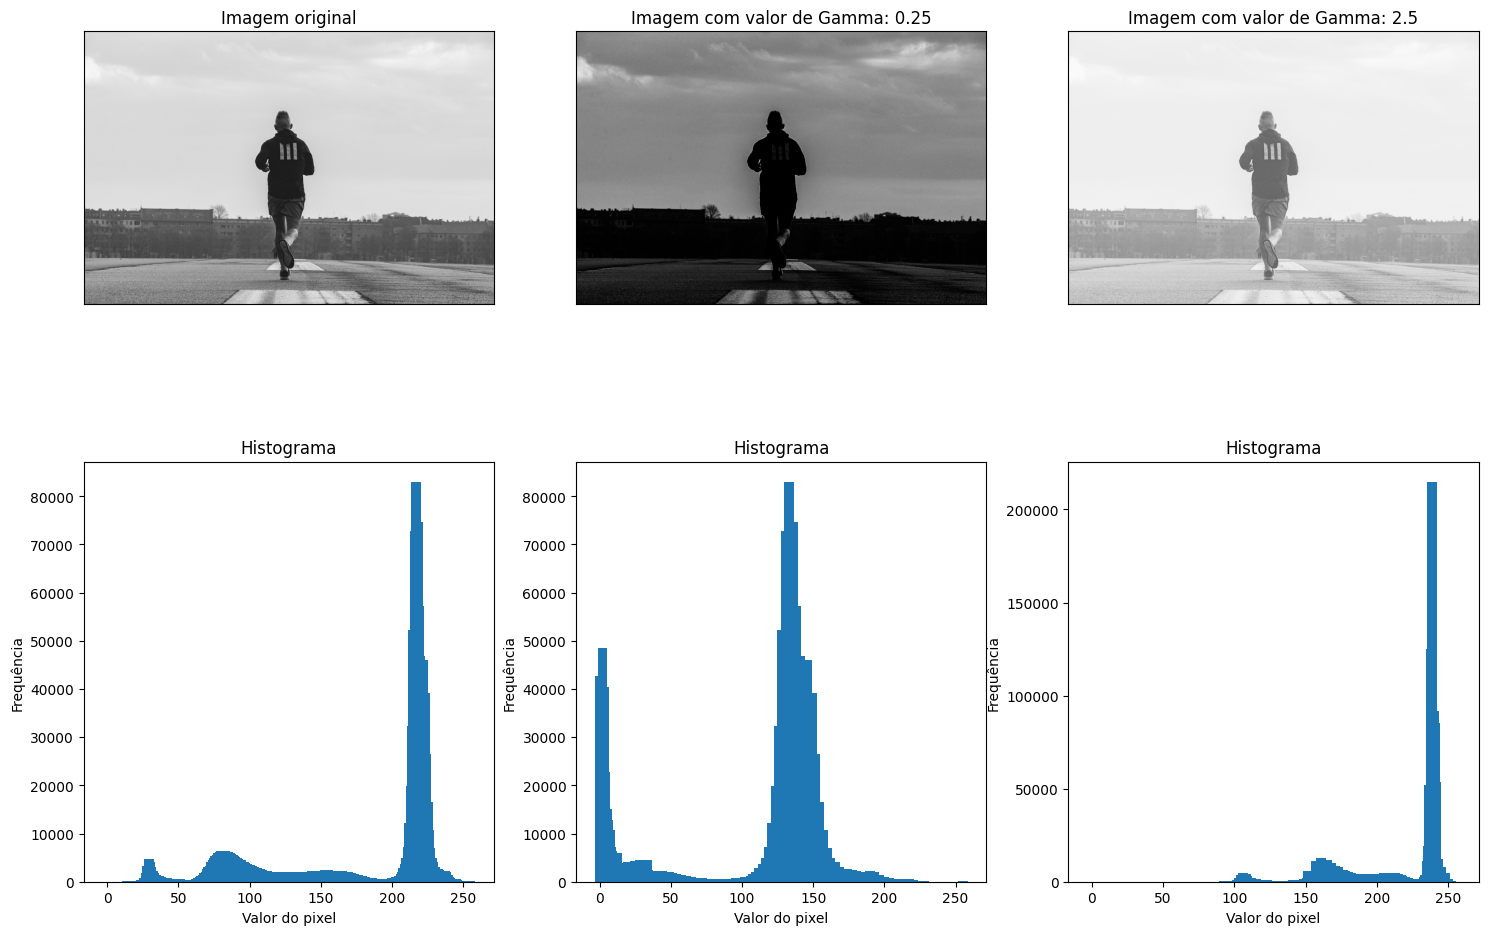
\includegraphics[width=1\linewidth]{Elementos/Figuras/resultados-gamma-runner.png}
    \caption{Imagem \textit{runner} em transformação por \textit{Gamma Correction}}
    \label{fig:gamma-runner}
\end{figure}

\begin{figure}
    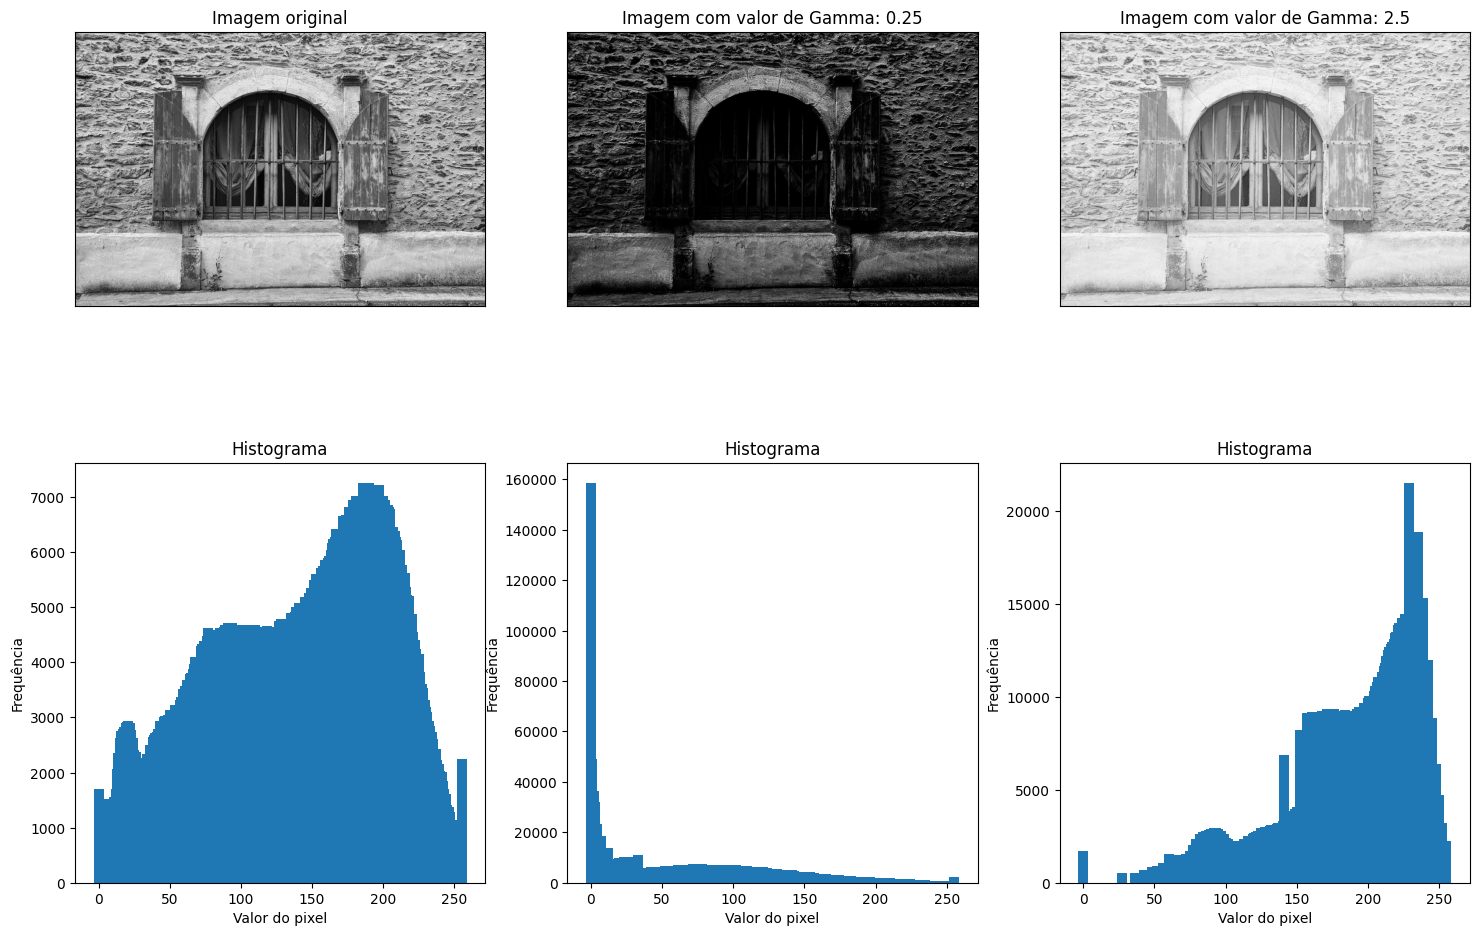
\includegraphics[width=1\linewidth]{Elementos/Figuras/resultados-gamma-shutters.png}
    \caption{Imagem \textit{shutters} em transformação por \textit{Gamma Correction}}
    \label{fig:gamma-shutters}
\end{figure}

\begin{figure}
    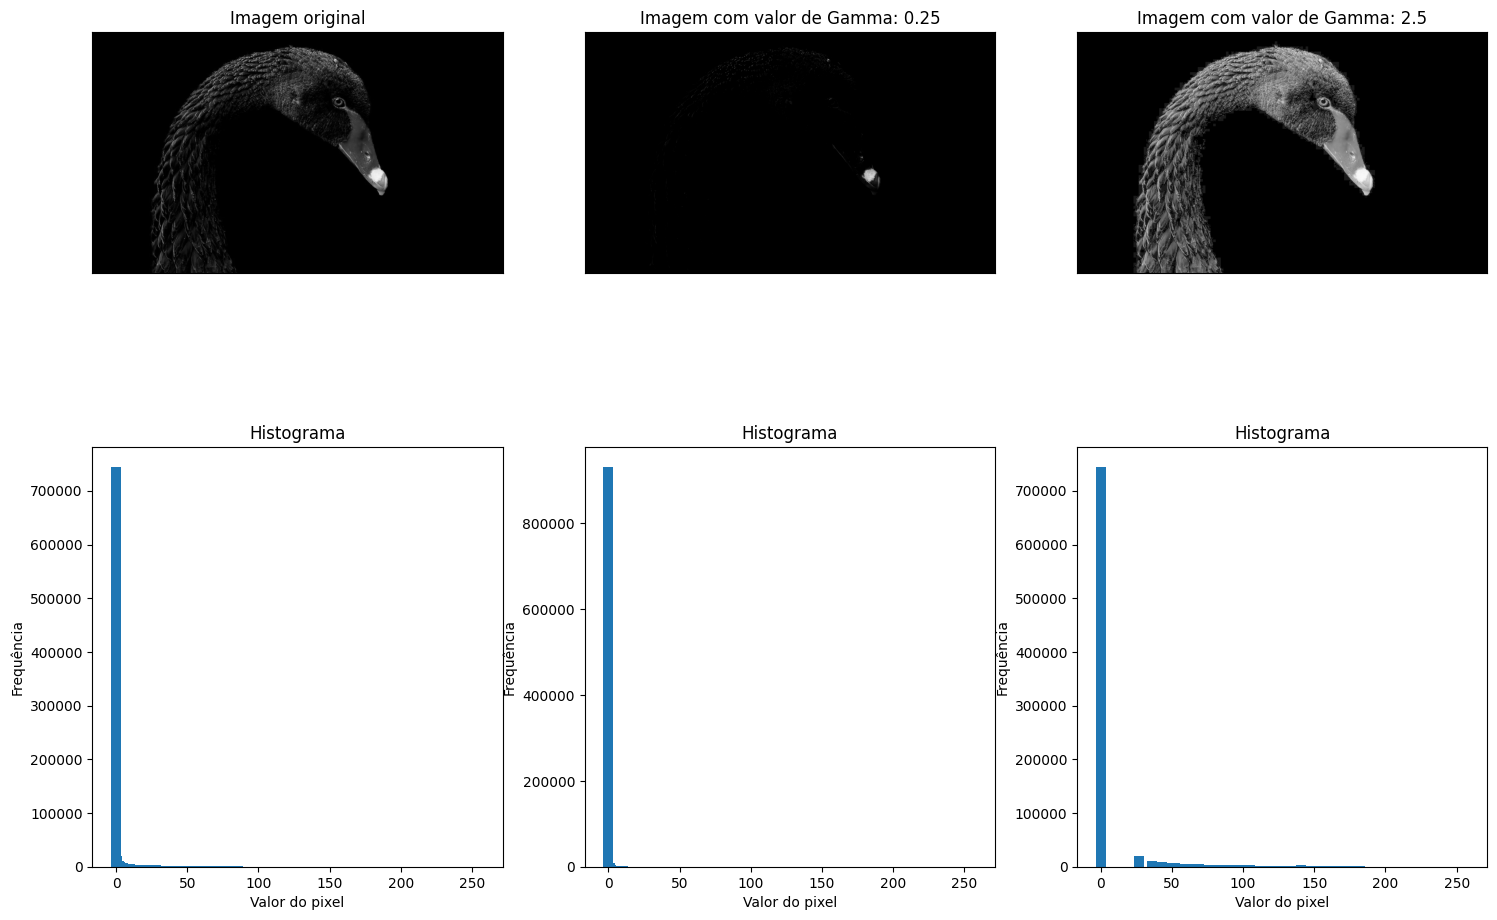
\includegraphics[width=1\linewidth]{Elementos/Figuras/resultados-gamma-swam.png}
    \caption{Imagem \textit{swan} em transformação por \textit{Gamma Correction}}
    \label{fig:gamma-swan}
\end{figure}

% -------------------------------------------------------------- %

\section{Binarização}

A binarização da imagem \textit{cairn} original e com os valores de \textit{gamma} $0.25$ e $2.5$ utilizando o limiar $127$ e o método \textit{Otsu} $157.0$, $67.0$ e $200.0$.
Conforme Figura \ref{fig:binarizacao-cairn}, podemos observar que na redução \textit{gamma} o resultado é uma imagem mais escura quando o valor de \textit{gamma} é $0.25$ e sendo o oposto quando o valor de \textit{gamma} é $2.5$.

\begin{figure}[h!]
    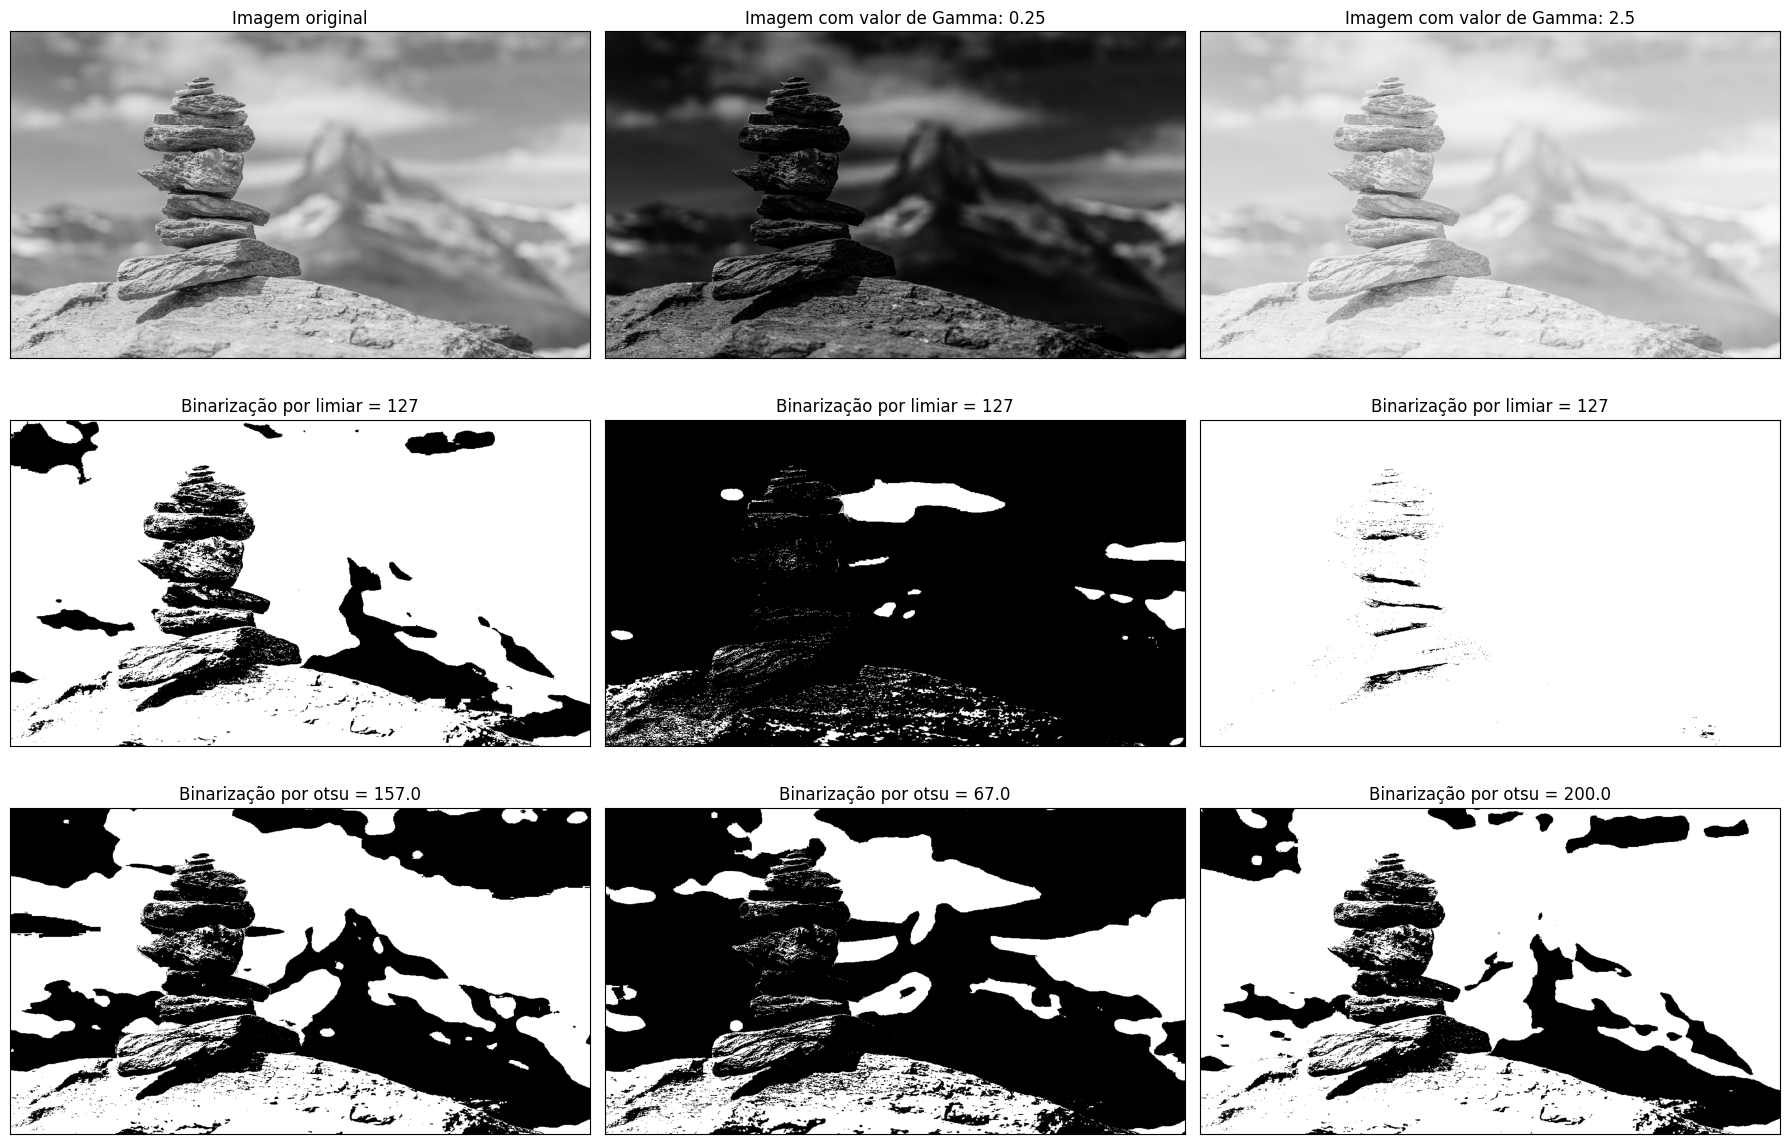
\includegraphics[width=1\linewidth]{Elementos/Figuras/resultados-binarizacao-cairn.png}
    \caption{Imagem \textit{cairn} em transformação por métodos de binarização}
    \label{fig:binarizacao-cairn}
\end{figure}

A binarização da imagem \textit{runner} original e com os valores de \textit{gamma} $0.25$ e $2.5$ utilizando o limiar $127$ e o método \textit{Otsu} $154.0$, $75.0$ e $199.0$.
Conforme Figura \ref{fig:binarizacao-runner}, podemos observar que na redução \textit{gamma} o resultado é uma imagem mais escura quando o valor de \textit{gamma} é $0.25$ e sendo o oposto quando o valor de \textit{gamma} é $2.5$.

\begin{figure}[h!]
    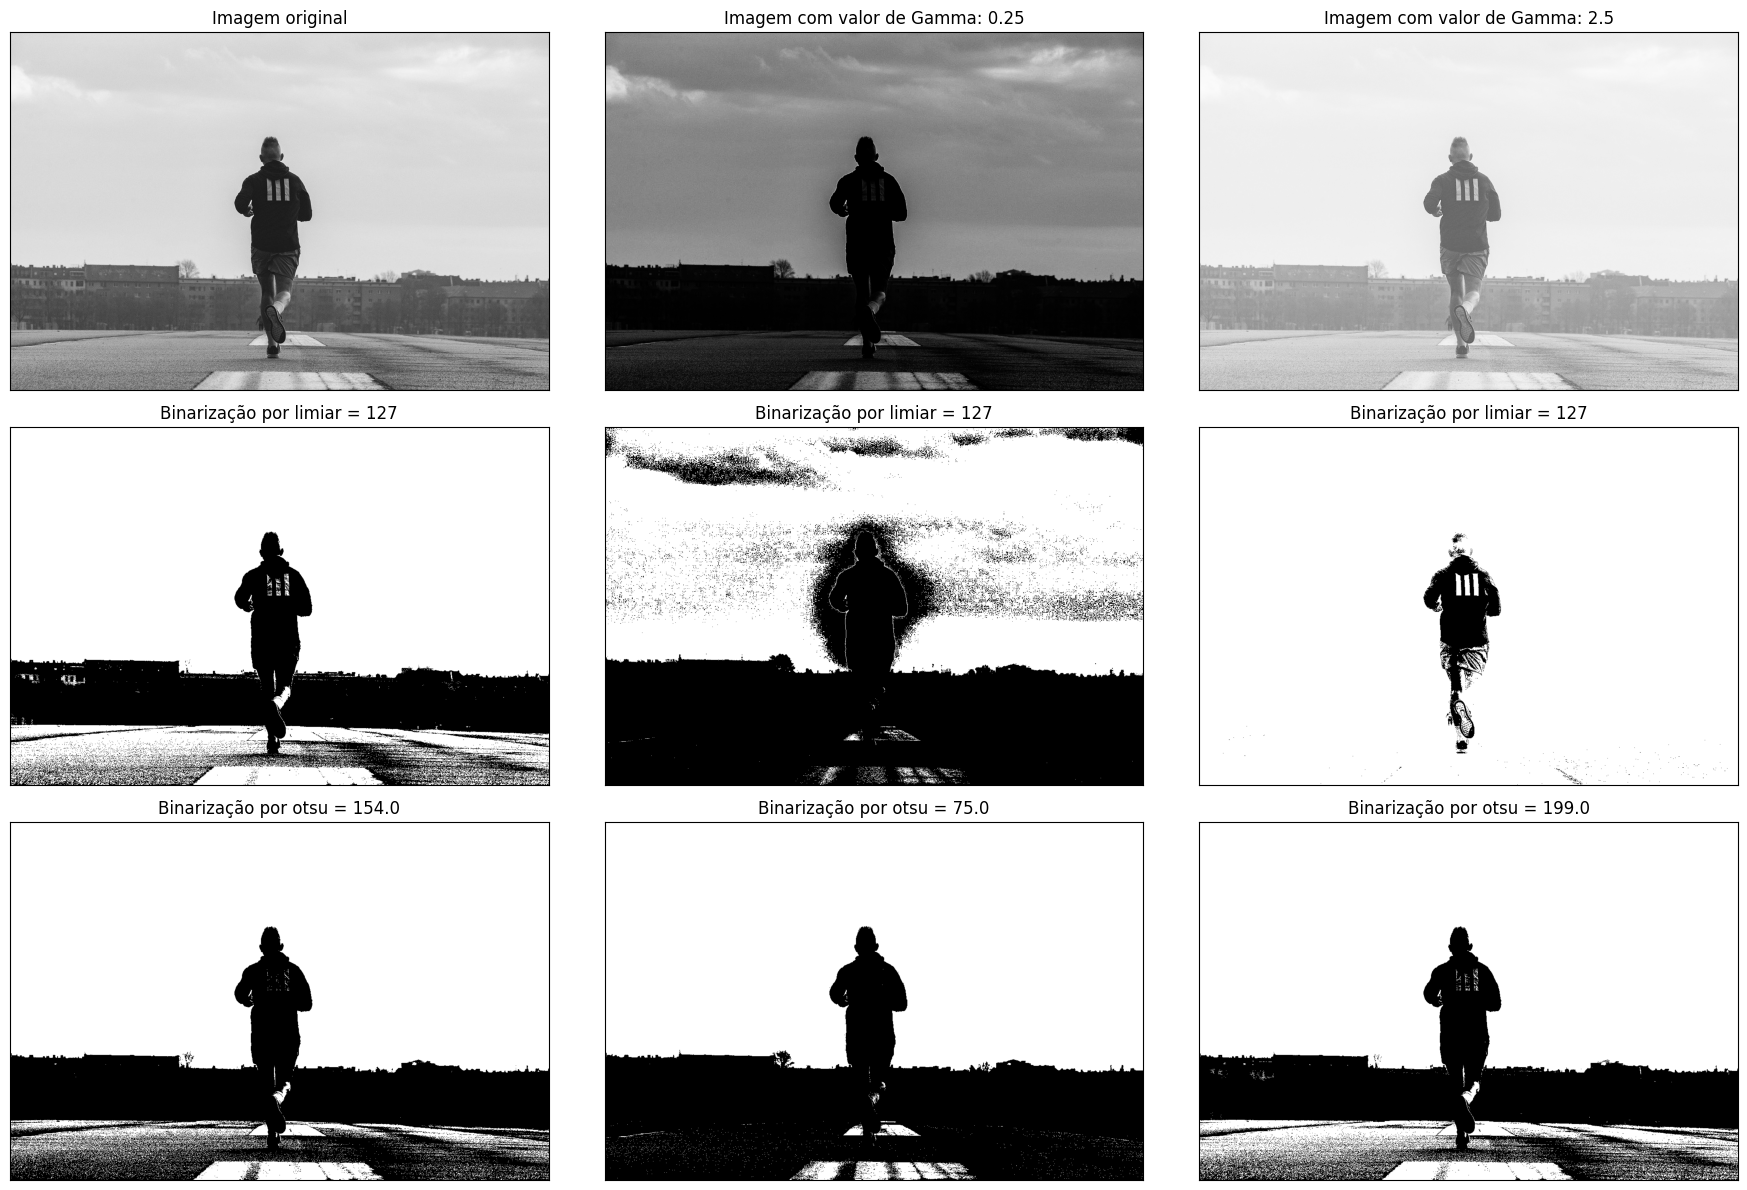
\includegraphics[width=1\linewidth]{Elementos/Figuras/resultados-binarizacao-runner.png}
    \caption{Imagem \textit{runner} em transformação por métodos de binarização}
    \label{fig:binarizacao-runner}
\end{figure}

Temos neste exemplo a imagem \textit{shutters} original e com os valores de \textit{gamma} $0.25$ e $2.5$ utilizando o limiar $127$ e o método \textit{Otsu} $130.0$, $70.0$ e $178.0$.
Conforme Figura \ref{fig:binarizacao-shutters}, observamos que na redução \textit{gamma} o resultado é uma imagem mais escura quando o valor de \textit{gamma} é $0.25$ e sendo o oposto quando o valor de \textit{gamma} é $2.5$.

\begin{figure}[h!]
    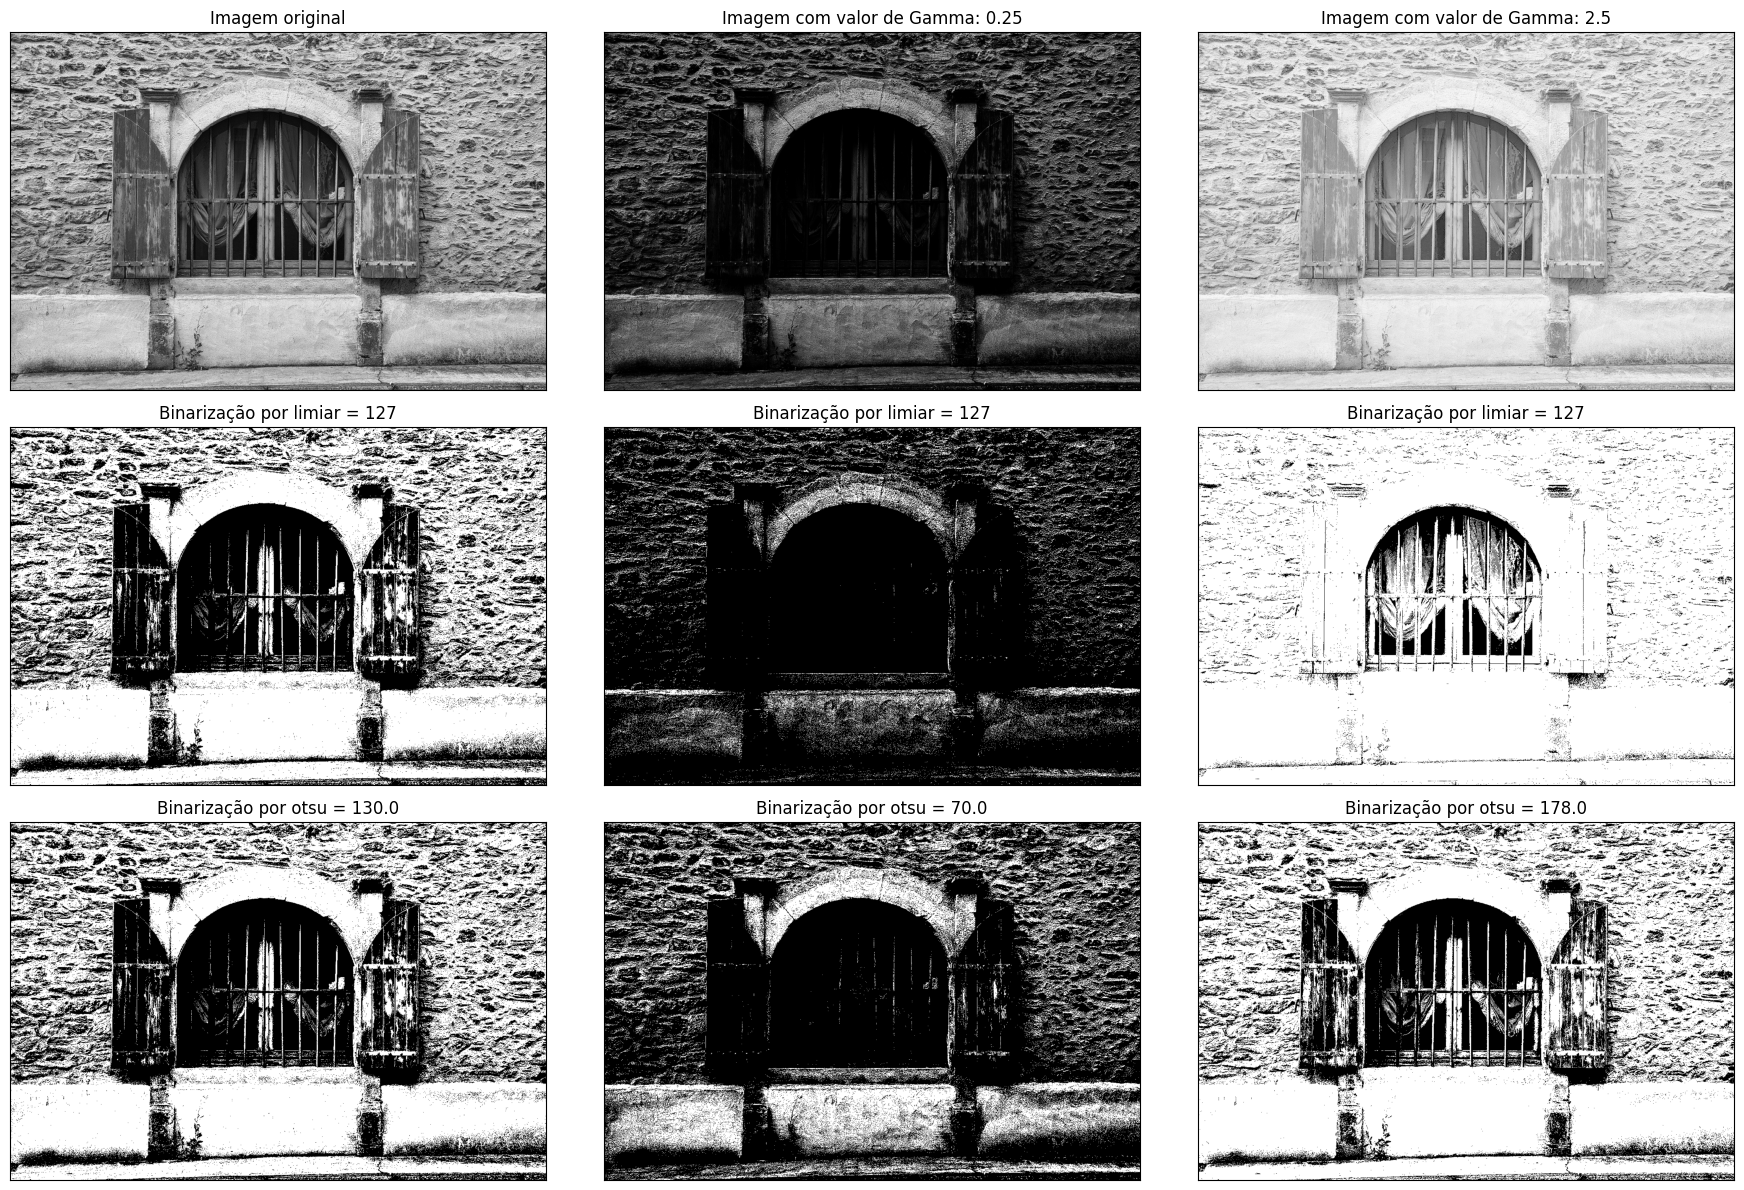
\includegraphics[width=1\linewidth]{Elementos/Figuras/resultados-binarizacao-shutters.png}
    \caption{Imagem \textit{shutters} em transformação por métodos de binarização}
    \label{fig:binarizacao-shutters}
\end{figure}

A binarização da imagem \textit{swan} original e com os valores de \textit{gamma} $0.25$ e $2.5$ utilizando o limiar $127$ e o método \textit{Otsu} $37.0$, $58.0$ e $76.0$.
Conforme Figura \ref{fig:binarizacao-swan}, podemos observar que na redução \textit{gamma} o resultado é uma imagem mais escura quando o valor de \textit{gamma} é $0.25$ e sendo o oposto quando o valor de \textit{gamma} é $2.5$.

\begin{figure}[h!]
    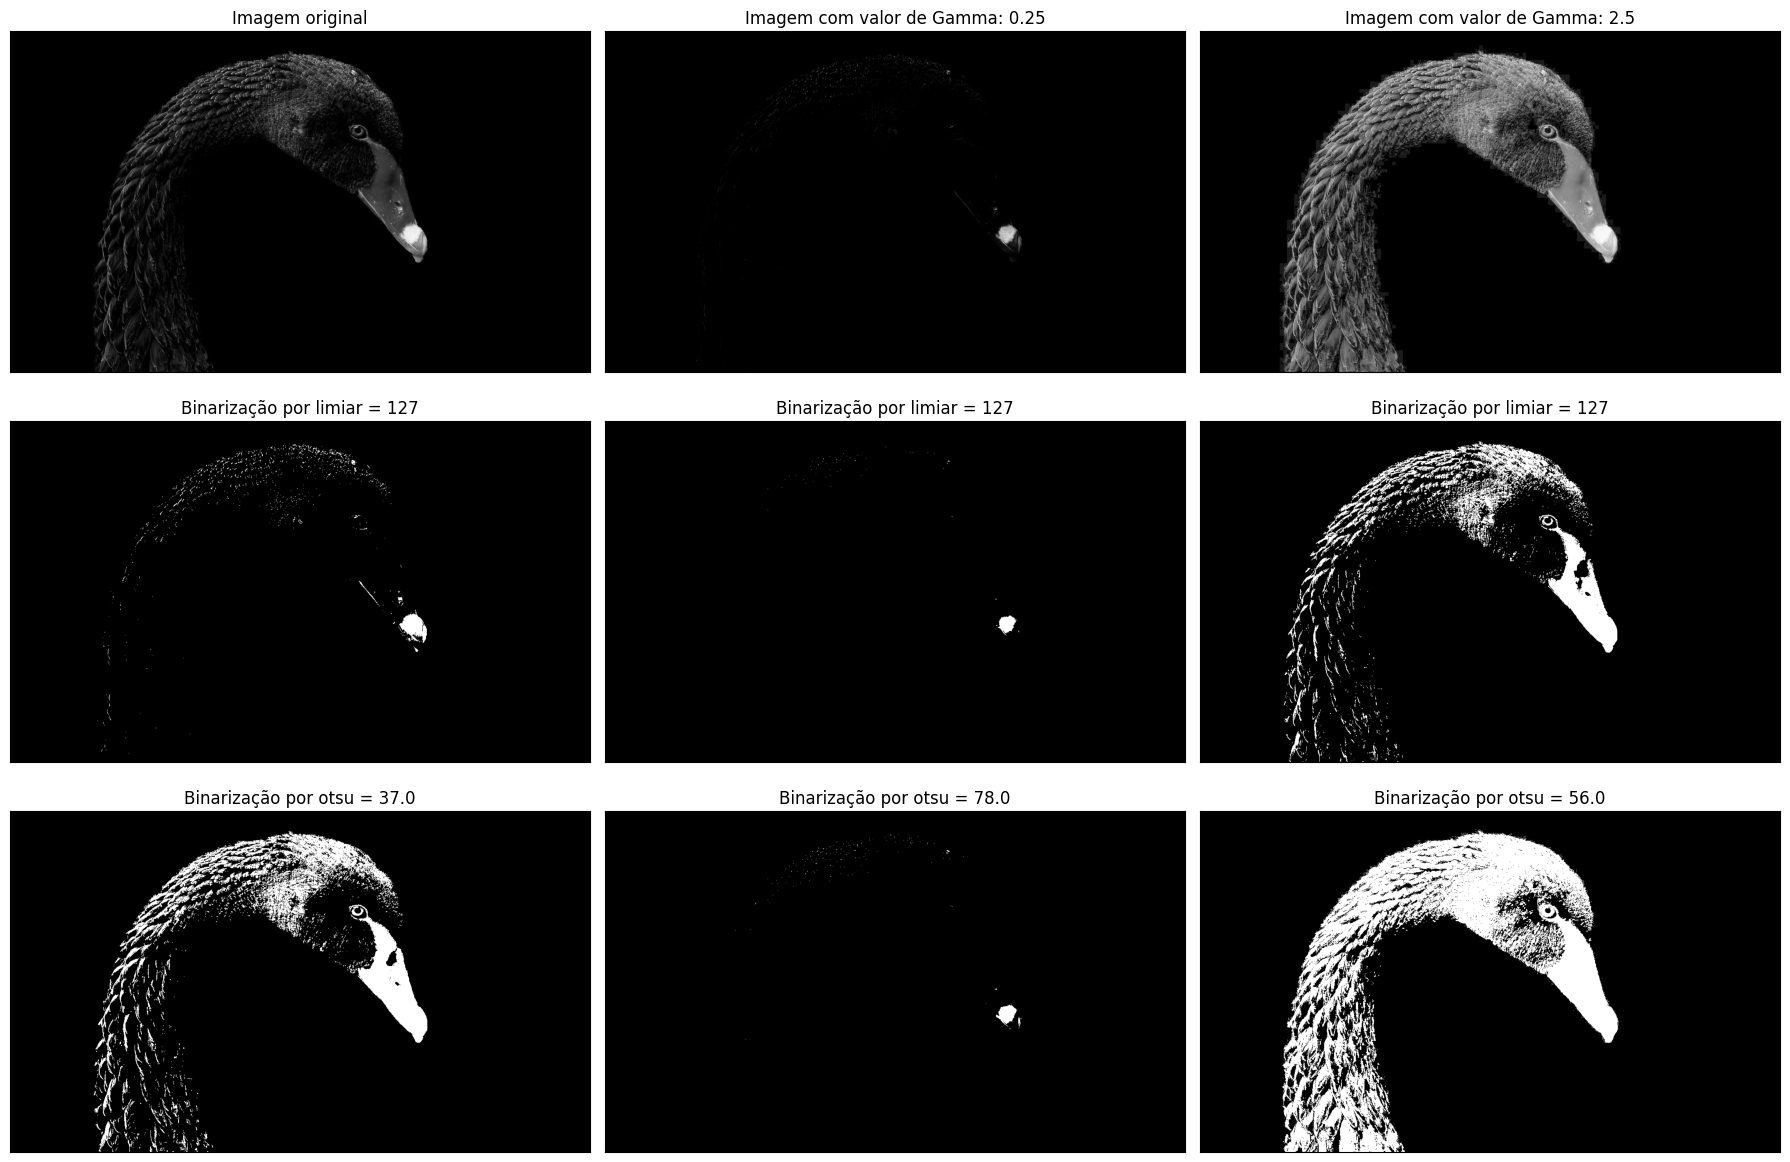
\includegraphics[width=1\linewidth]{Elementos/Figuras/resultados-binarizacao-swan.png}
    \caption{Imagem \textit{swan} em transformação por métodos de binarização}
    \label{fig:binarizacao-swan}
\end{figure}

% -------------------------------------------------------------- %

\section{Modificação de \textit{bits} menos e mais significativos}

Conforme proposto, foram zerados os LSBs e os MSBs das imagens utilizadas nesta atividade a fim de realizar análises acerca da quantidade máxima de \textit{bits} mais e menos significativos que podem ser utilizados para a ocultação de informações.

\subsection{Comparação dos histogramas das imagens com LSBs zerados}

As imagens com 1, 2, 3, 4, 5, 6 e 7 LSBs (Figuras \ref{fig:swan-lsb} a \ref{fig:cairn-lsb})foram dispostas lado a lado.  Ao lado de cada imagem está o seu histograma, por meio do qual pode-se observar a diminuição do número de tonalidades conforme a quantidade de LSBs aumenta. 

\begin{figure}[h!]
    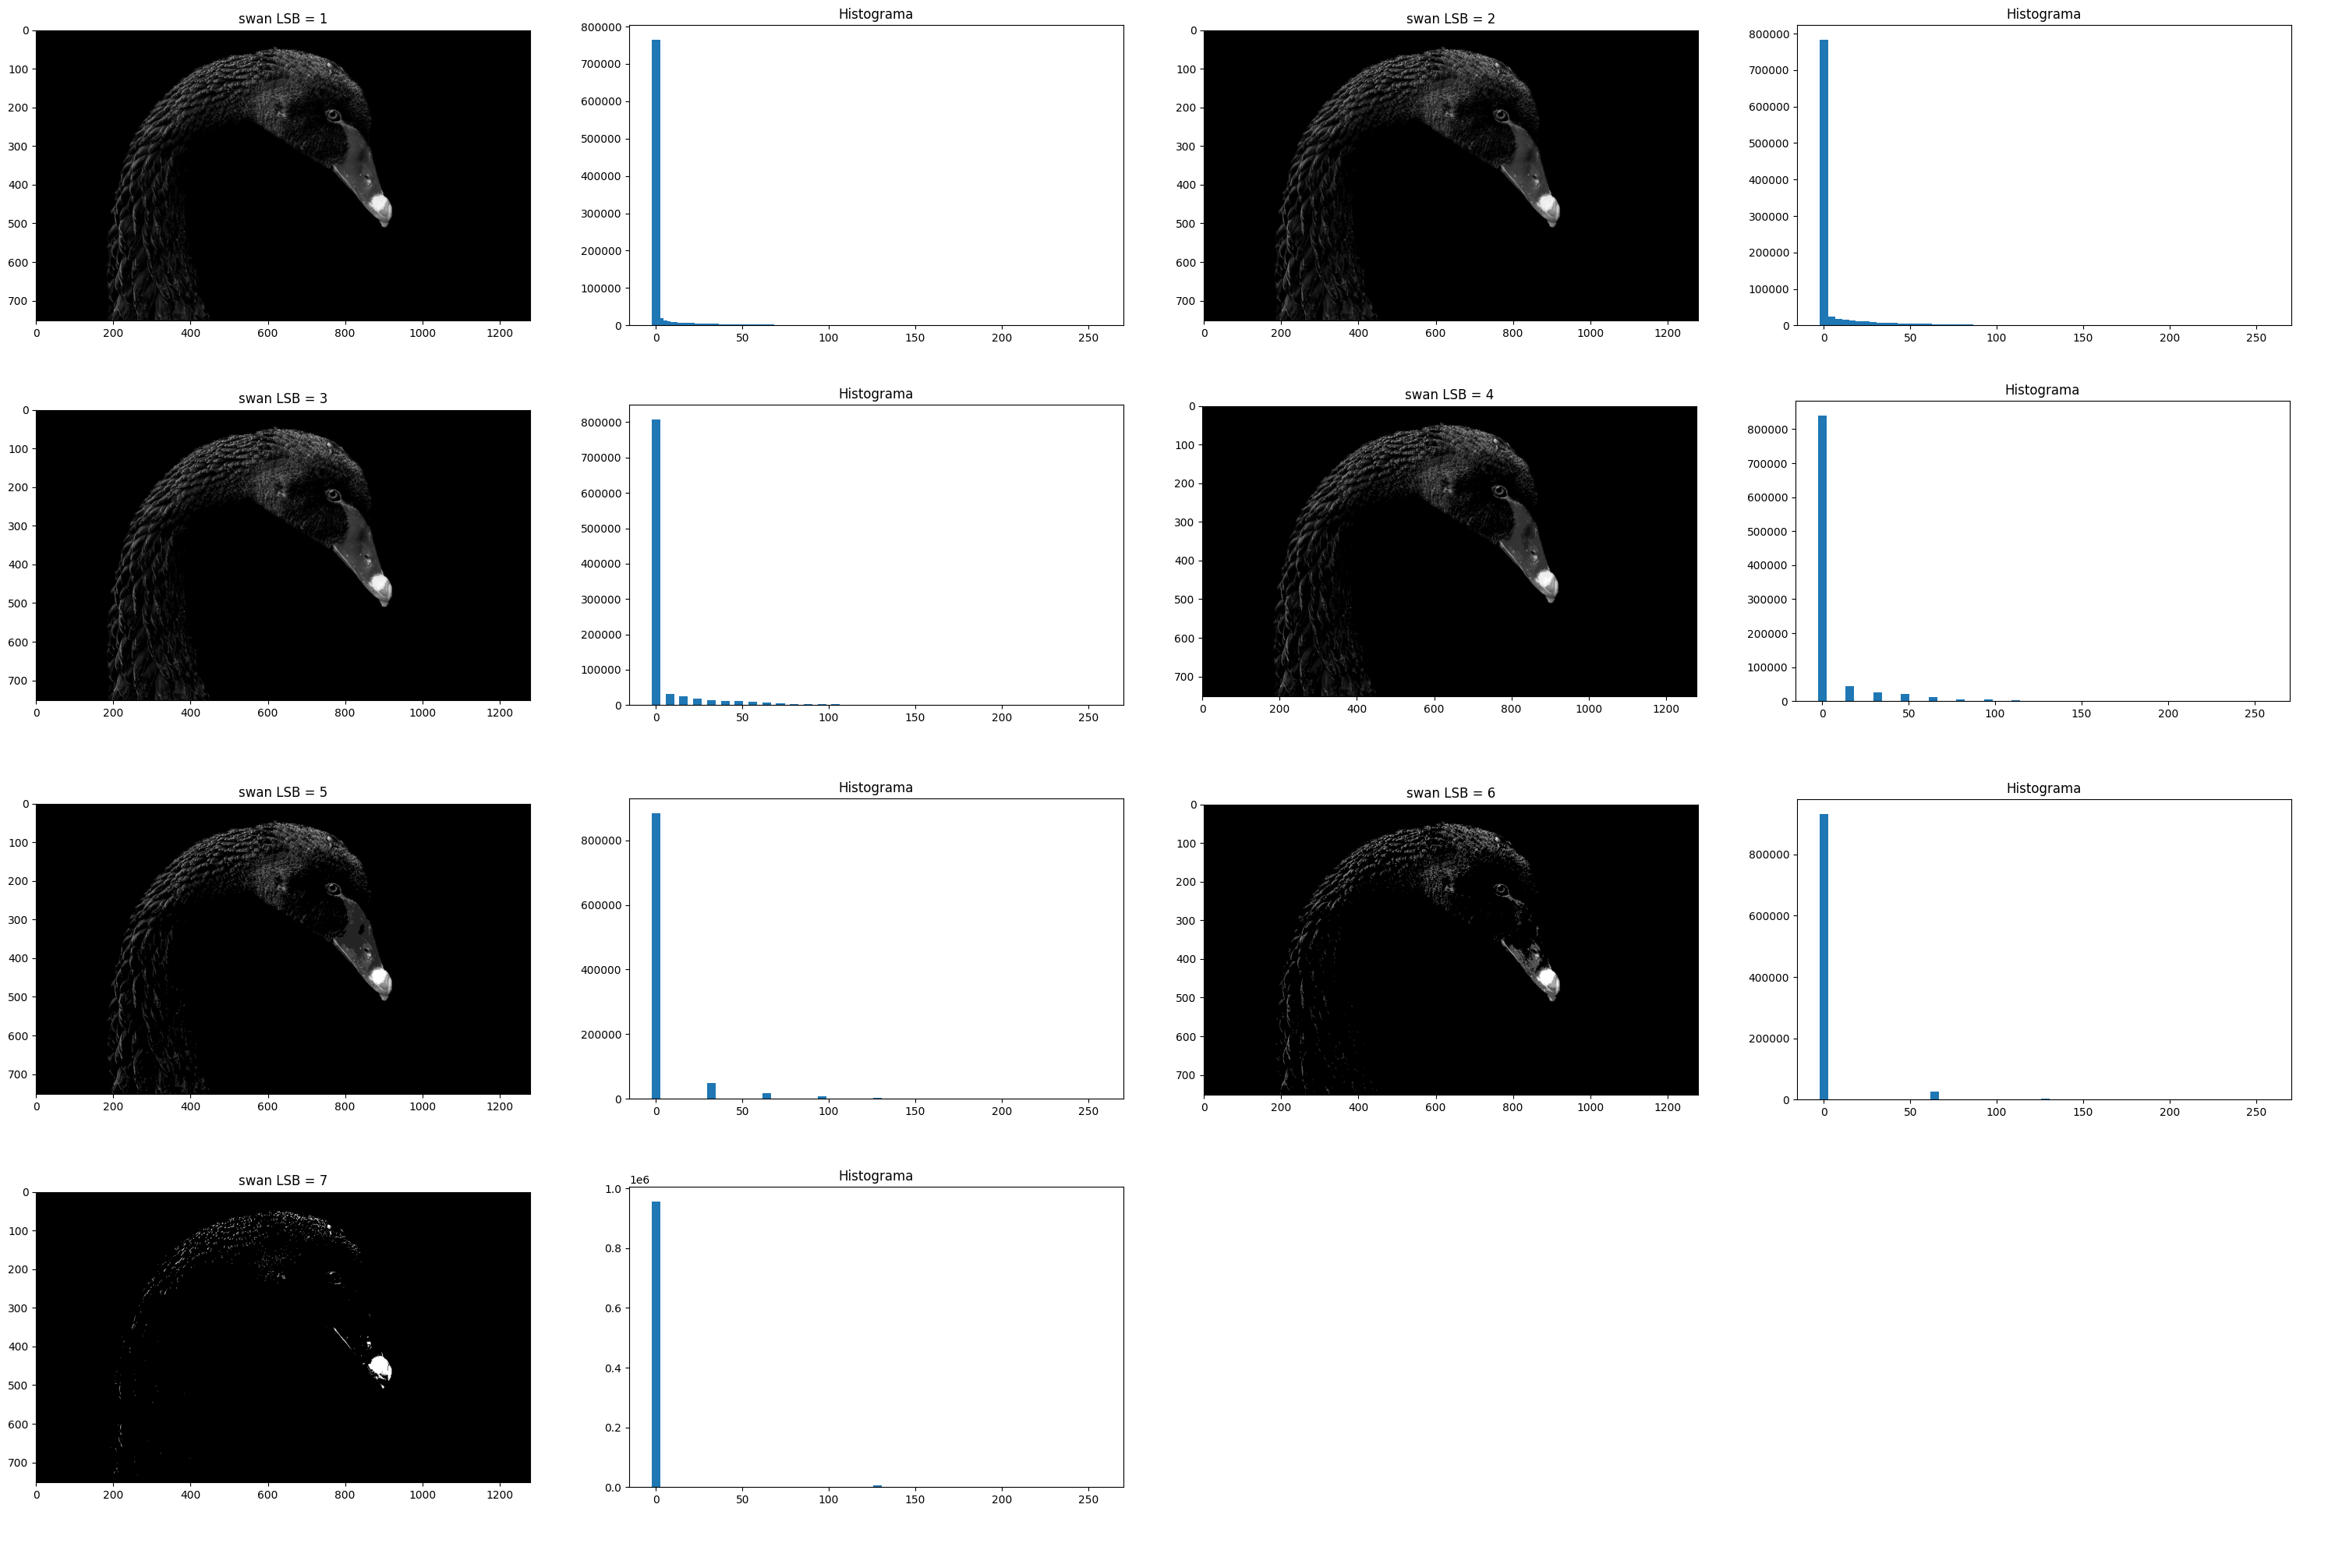
\includegraphics[width=1\linewidth]{Elementos//Figuras/swan_lsb.png}
    \caption{Da esquerda para a direita e de cima para baixo temos: Imagem Swan com 1, 2, 3, 4, 5, 6 e 7 LSBs zerados.}
    \label{fig:swan-lsb}
\end{figure}

Ao observar os histogramas da imagem \textit{swan} (Figura \ref{fig:swan-lsb}), percebe-se que a diminuição da quantidade de tonalidades não é tão notável como nas demais imagens, isso ocorre pois a imagem original não apresenta grande variação em seus níveis de cinza, além de apresentar uma única tonalidade com frequência muito mais alta do que as demais.

\begin{figure}[h!]
    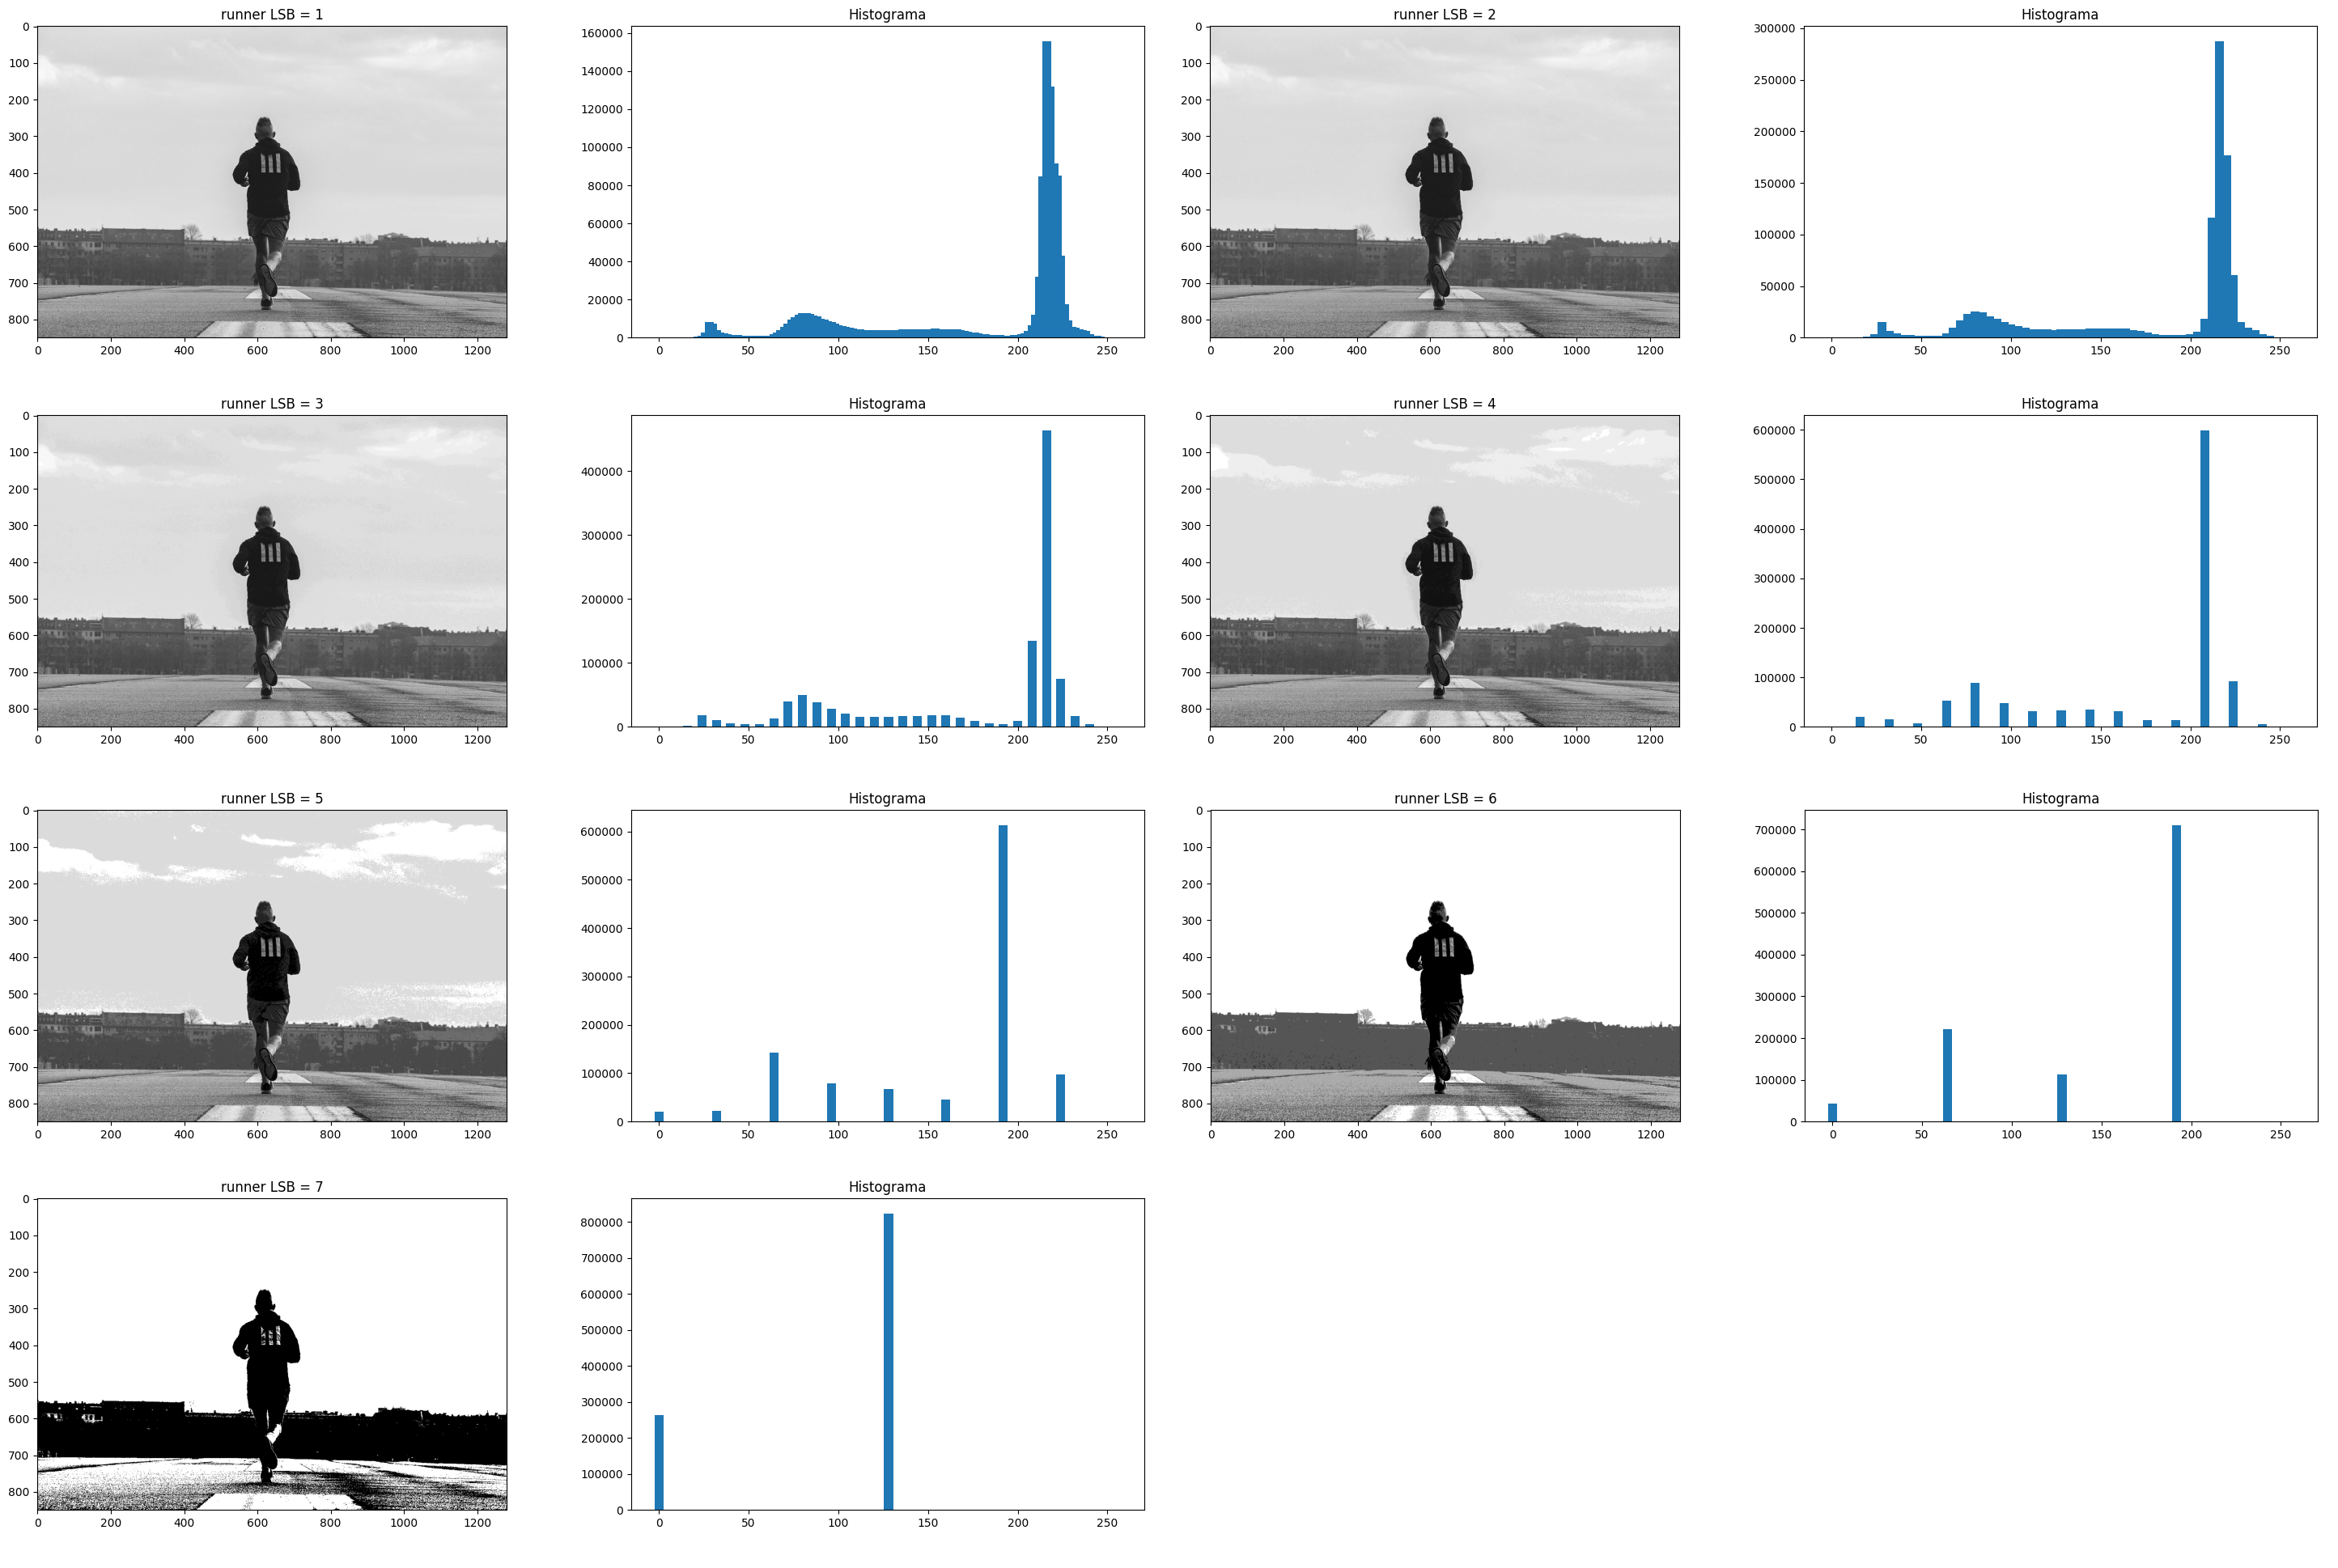
\includegraphics[width=1\linewidth]{Elementos//Figuras/runner_lsb.png}
    \caption{Da esquerda para a direita e de cima para baixo temos: Imagem Runner com 1, 2, 3, 4, 5, 6 e 7 LSBs zerados.}
    \label{fig:runner-lsb}
\end{figure}

\begin{figure}[h!]
    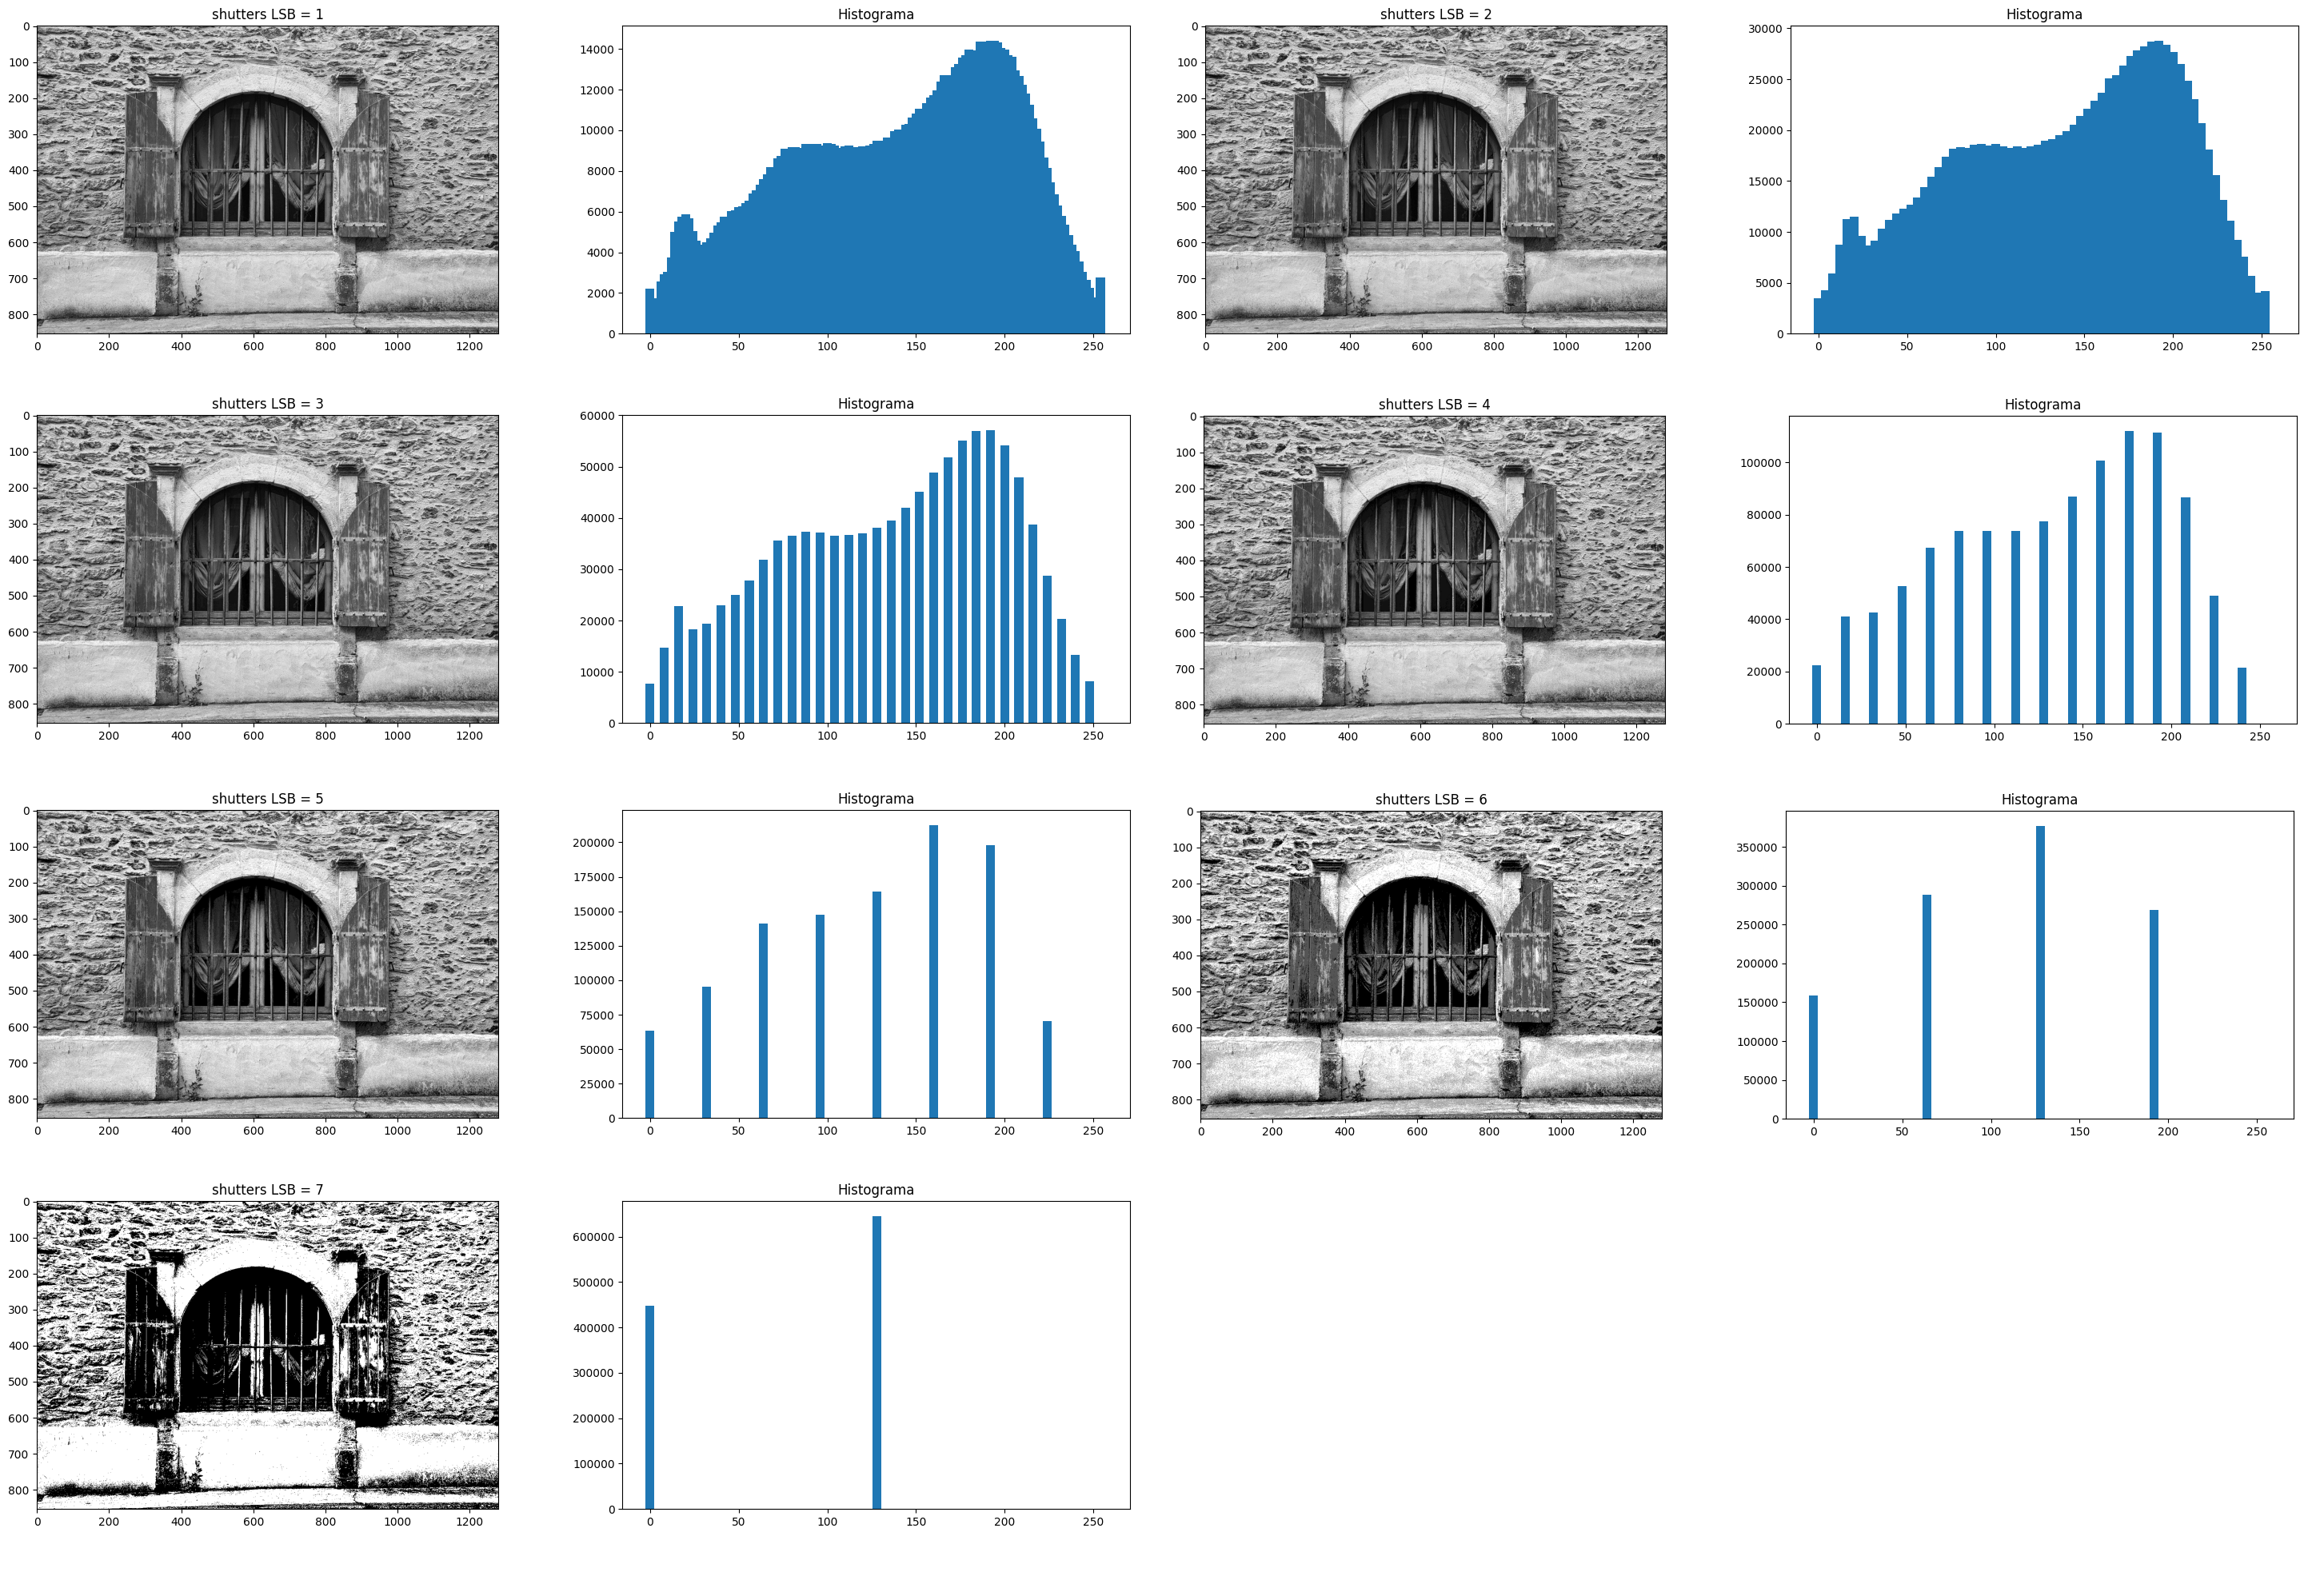
\includegraphics[width=1\linewidth]{Elementos//Figuras/shutters_lsb.png}
    \caption{Da esquerda para a direita e de cima para baixo temos: Imagem Shutters com 1, 2, 3, 4, 5, 6 e 7 LSBs zerados.}
    \label{fig:shutters-lsb}
\end{figure}

\begin{figure}[h!]
    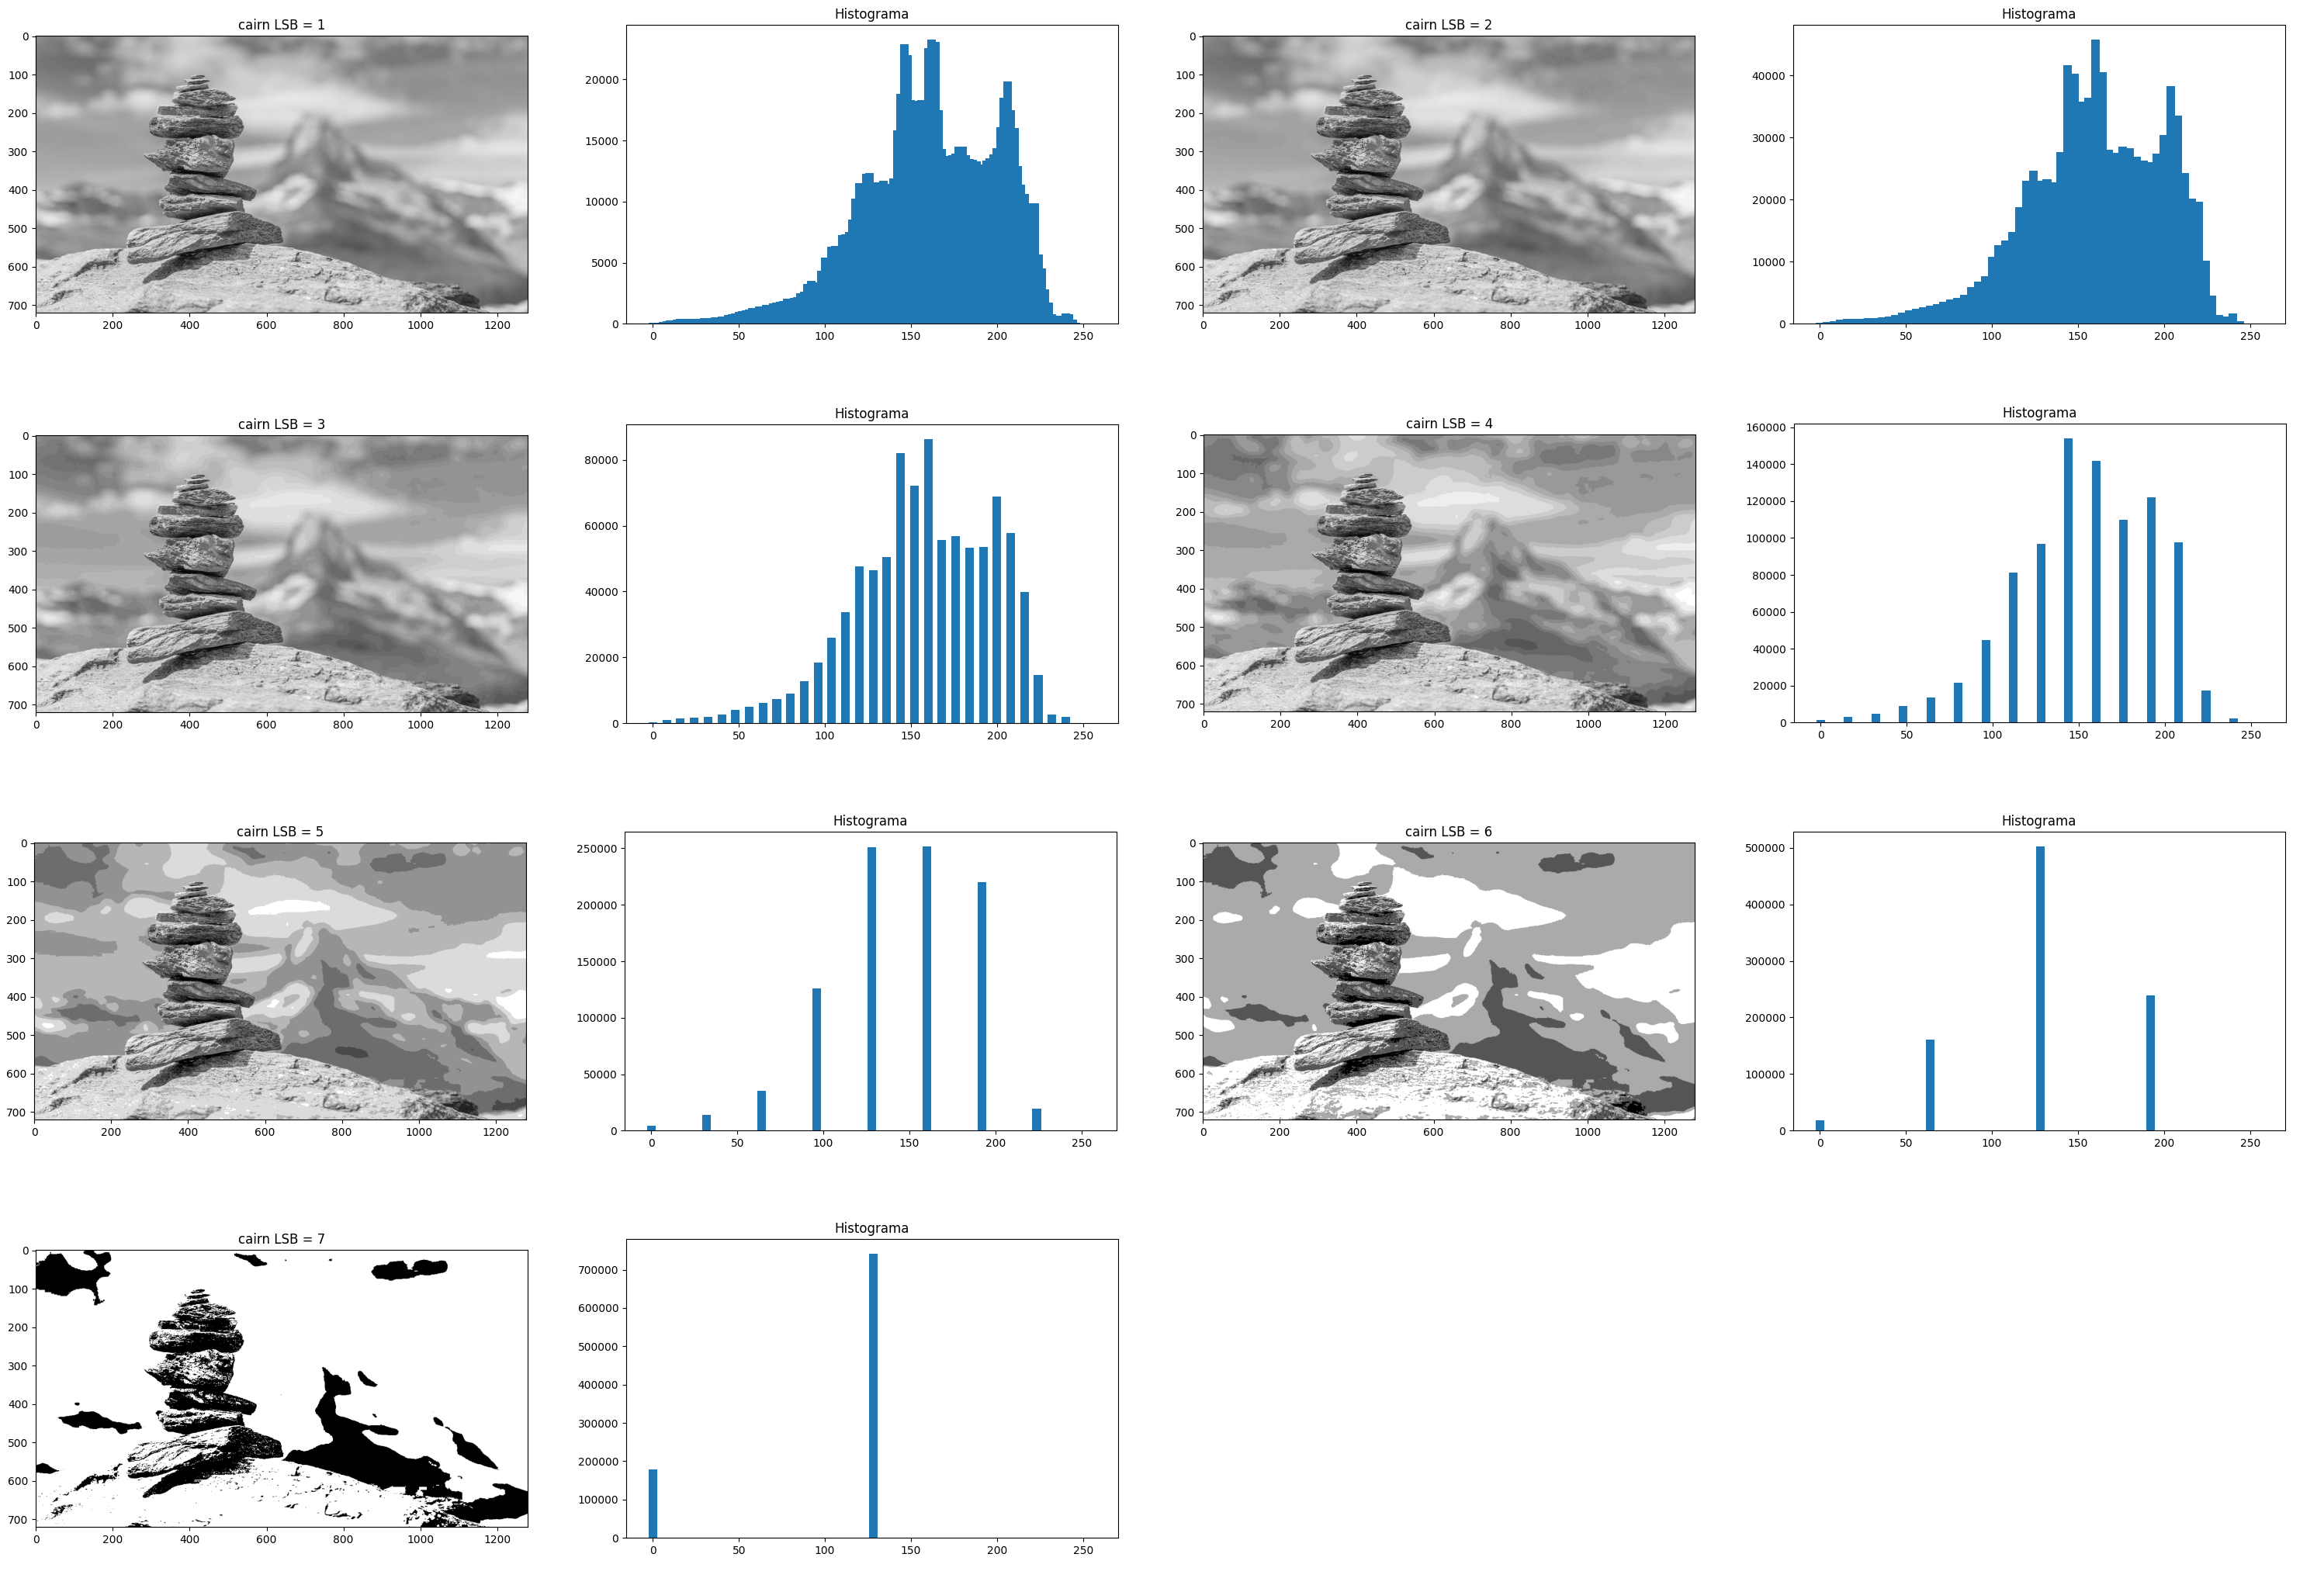
\includegraphics[width=1\linewidth]{Elementos//Figuras/cairn_lsb.png}
    \caption{Da esquerda para a direita e de cima para baixo temos: Imagem Cairn com 1, 2, 3, 4, 5, 6 e 7 LSBs zerados.}
    \label{fig:cairn-lsb}
\end{figure}

Ao realizar uma análise subjetiva das imagens modificadas, percebe-se que todas as imagens, com exceção da imagem \textit{shutters} (Figura \ref{fig:shutters-lsb}), não apresentam ruídos visualmente perceptíveis quando se utiliza até 4 LSBs para ocultação de informações. A imagem \textit{shutters}, por sua vez, não apresenta grandes distorções utilizando até 5 LSBs.

% ---------------------------------------------------------------- %

\subsection{Comparação dos histogramas das imagens com MSBs zerados}

Semelhante ao que foi feito nos experimentos com os LSBs, as imagens com 1, 2, 3, 4, 5, 6 e 7 MSBs (Figuras \ref{fig:swan-msb} a \ref{fig:cairn-msb}) foram dispostas lado a lado. Ao lado de cada imagem está o seu histograma, por meio do qual pode-se observar a diminuição do número de tonalidades conforme a quantidade de MSBs aumenta. 

\begin{figure}[h!]
    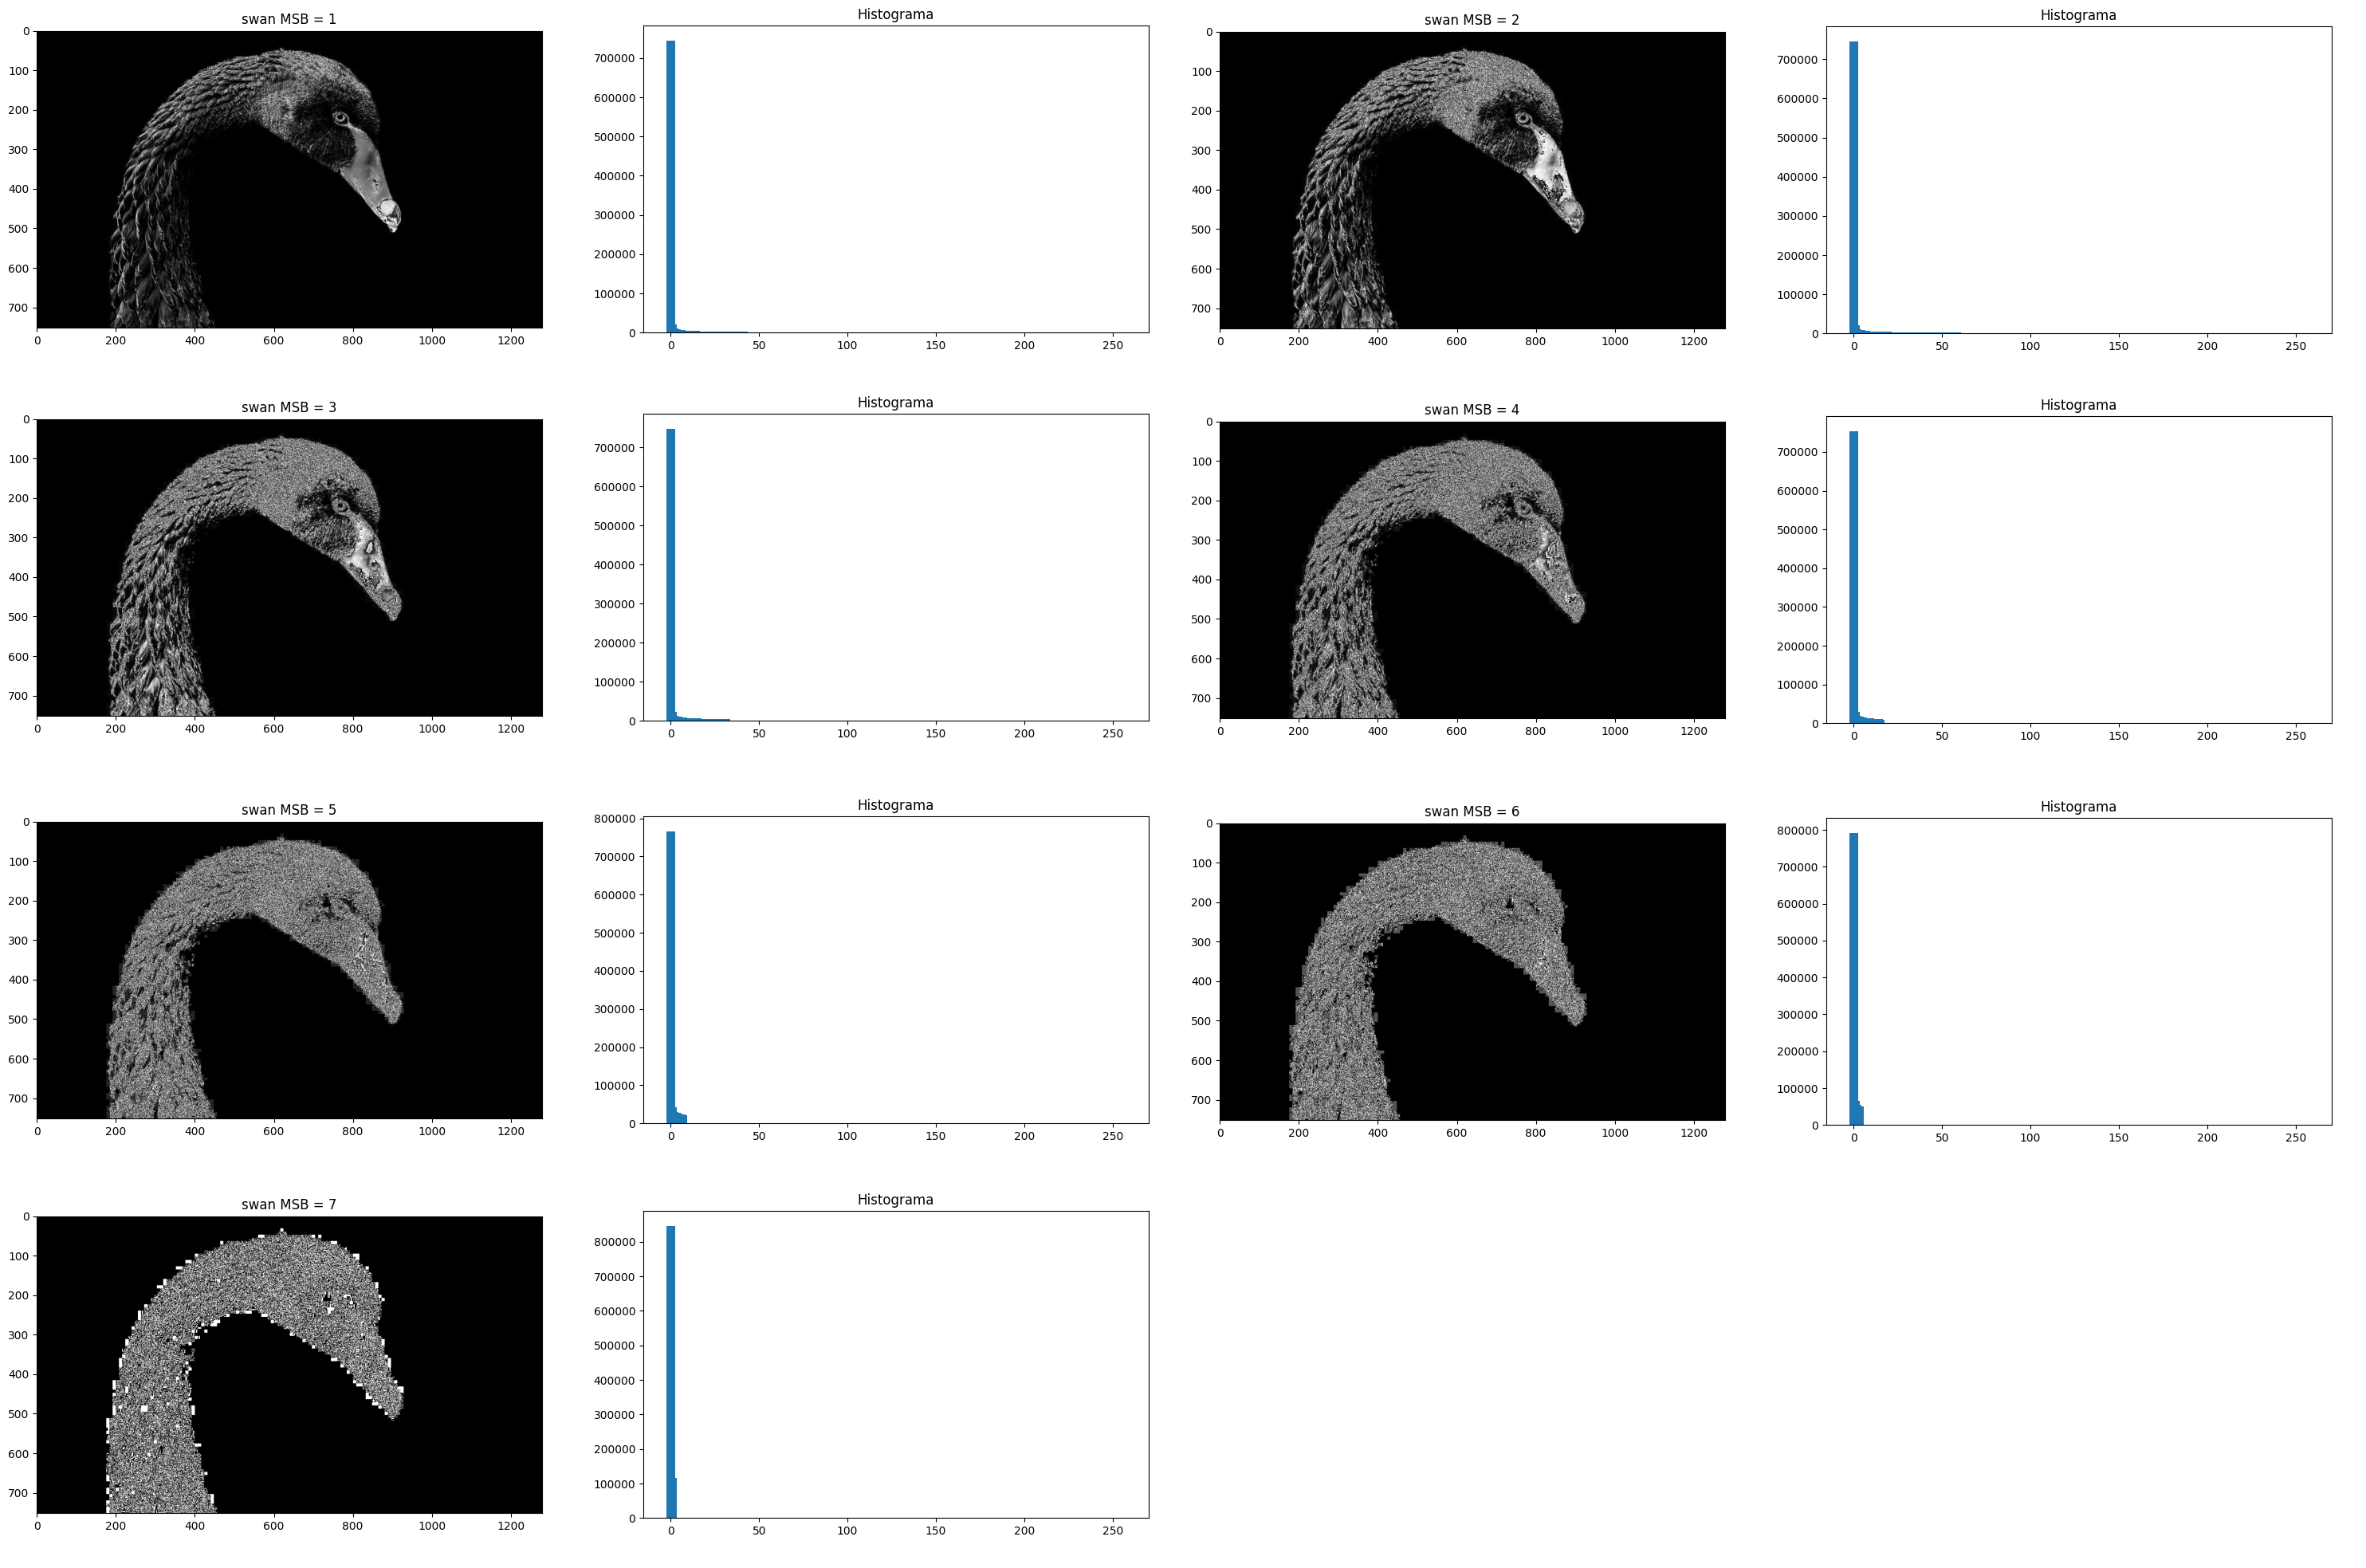
\includegraphics[width=1\linewidth]{Elementos//Figuras/swan_msb.png}
    \caption{Da esquerda para a direita e de cima para baixo temos: Imagem Swan com 1, 2, 3, 4, 5, 6 e 7 MSBs zerados.}
    \label{fig:swan-msb}
\end{figure}

\begin{figure}[h!]
    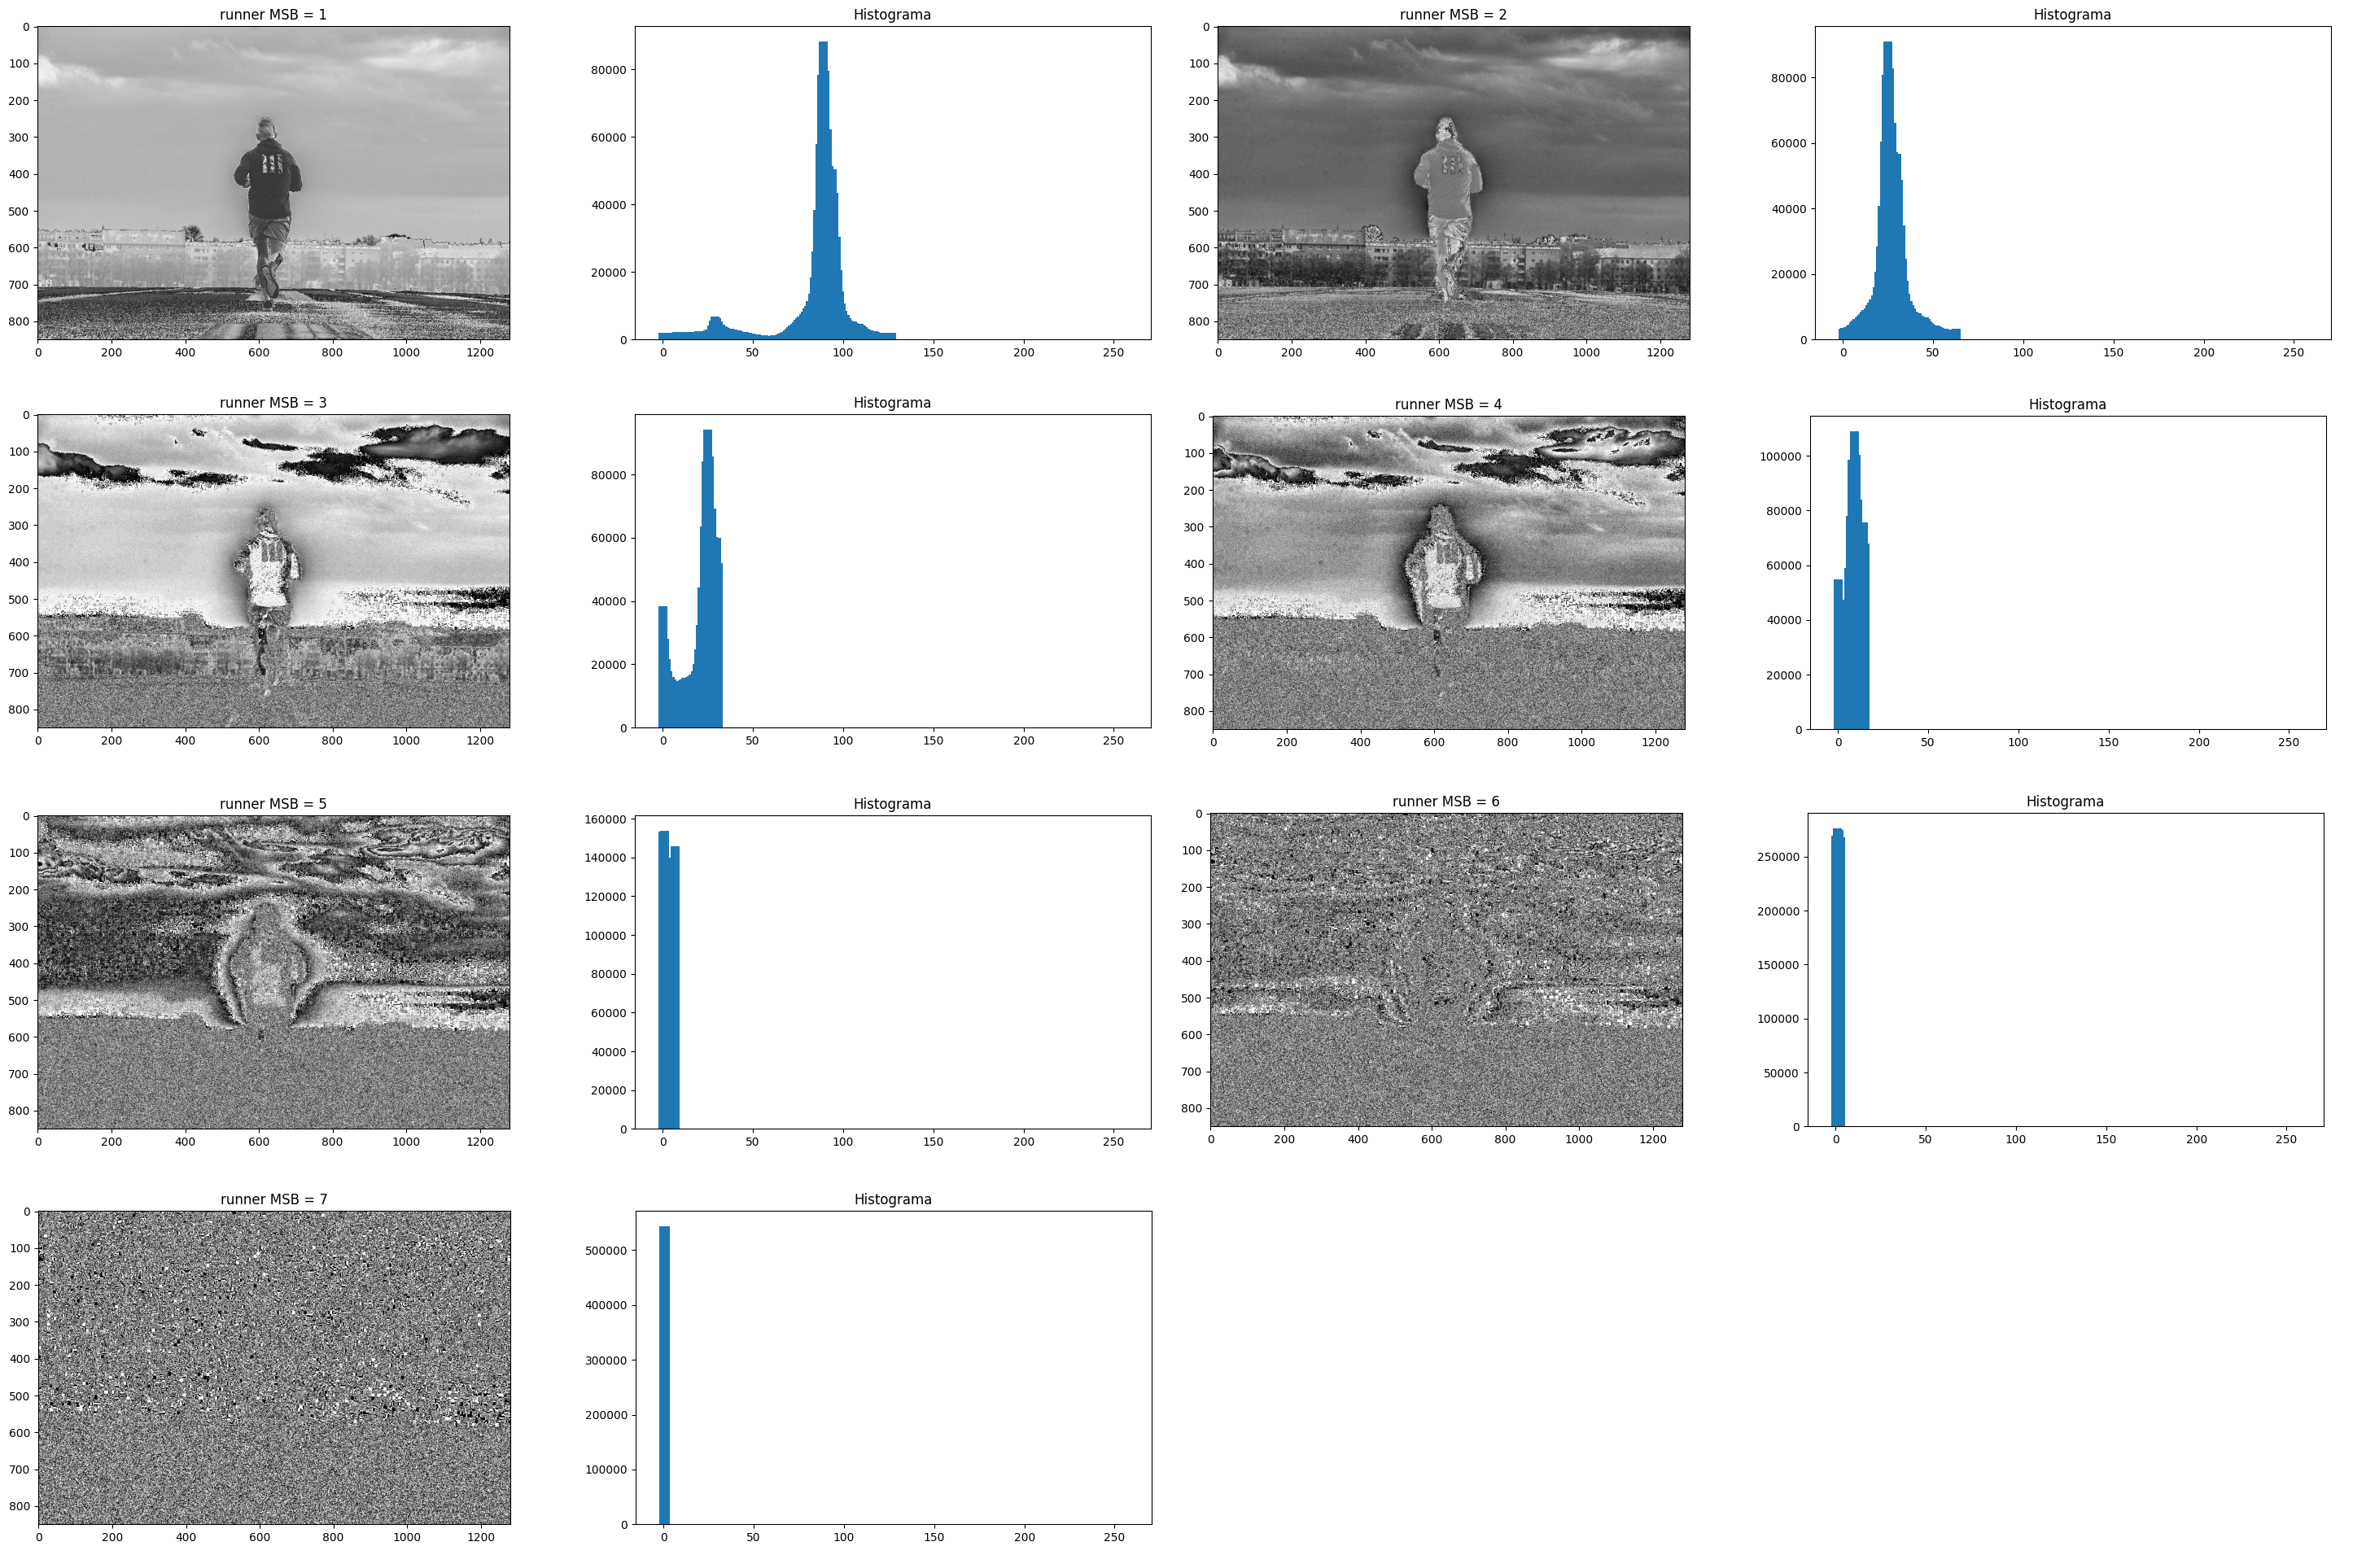
\includegraphics[width=1\linewidth]{Elementos//Figuras/runner_msb.png}
    \caption{Da esquerda para a direita e de cima para baixo temos: Imagem Runner com 1, 2, 3, 4, 5, 6 e 7 MSBs zerados.}
    \label{fig:runner-msb}
\end{figure}

\begin{figure}[h!]
    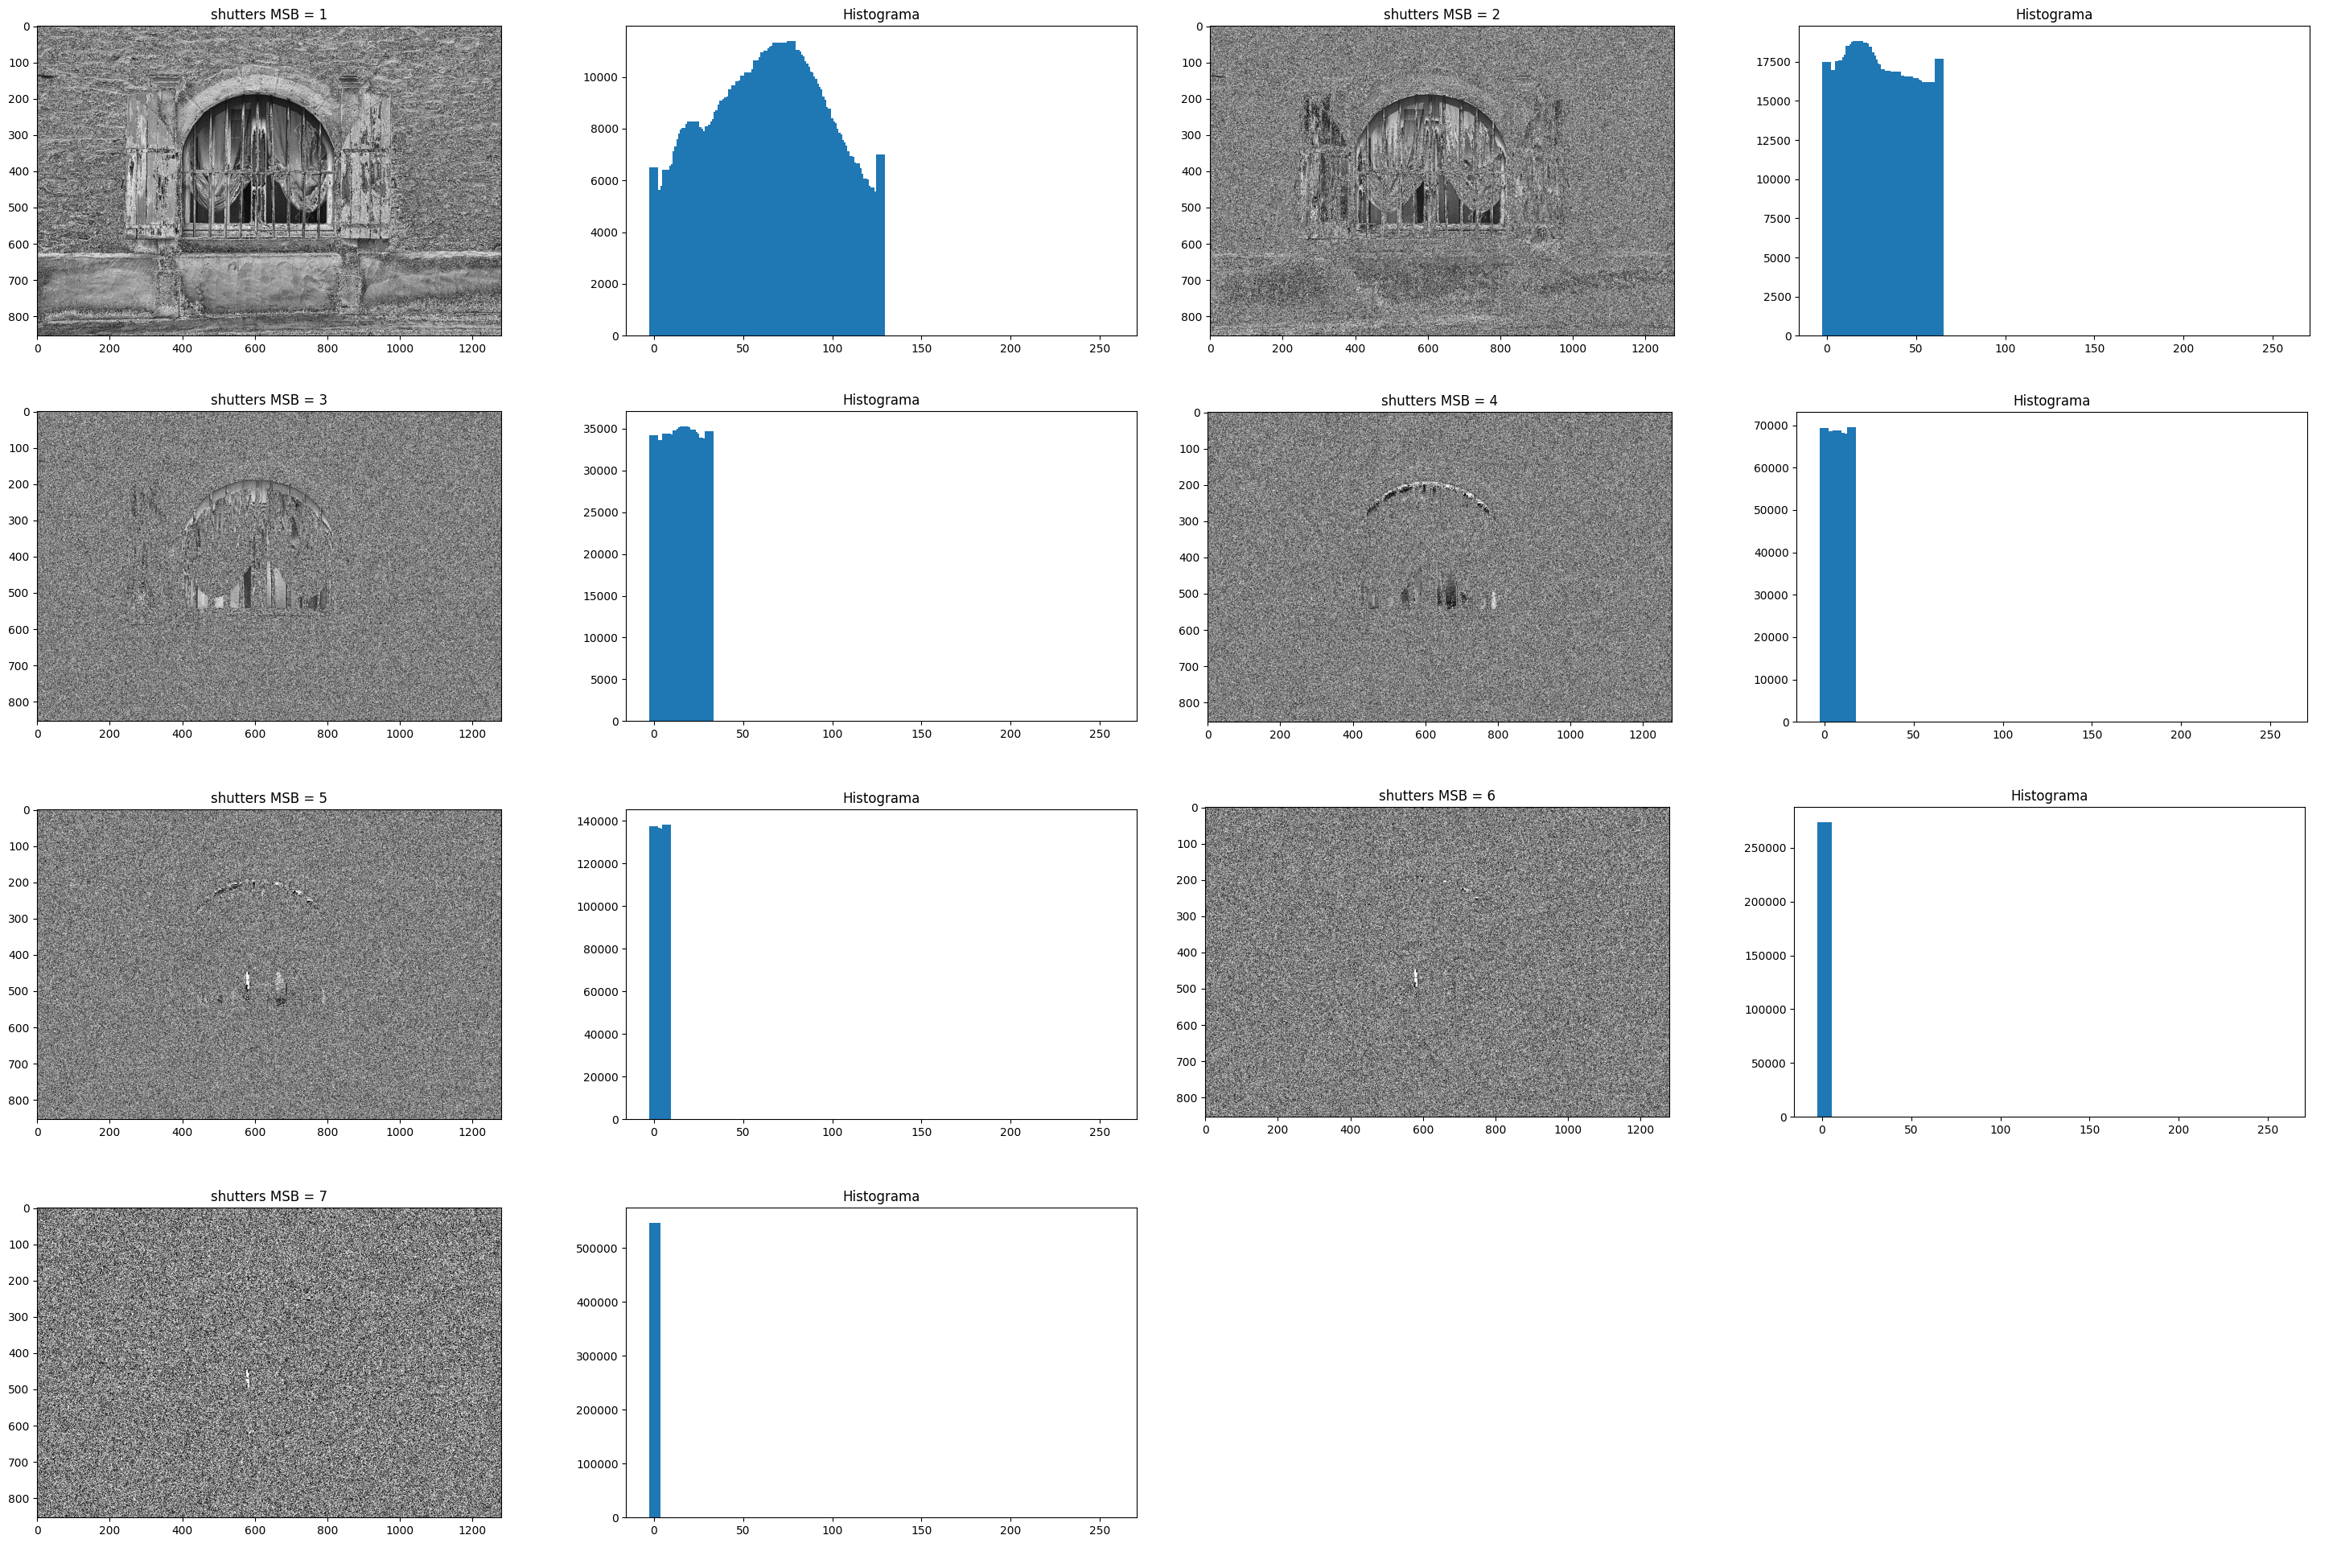
\includegraphics[width=1\linewidth]{Elementos//Figuras/shutters_msb.png}
    \caption{Da esquerda para a direita e de cima para baixo temos: Imagem Shutters com 1, 2, 3, 4, 5, 6 e 7 MSBs zerados.}
    \label{fig:shutters-msb}
\end{figure}

\begin{figure}[h!]
    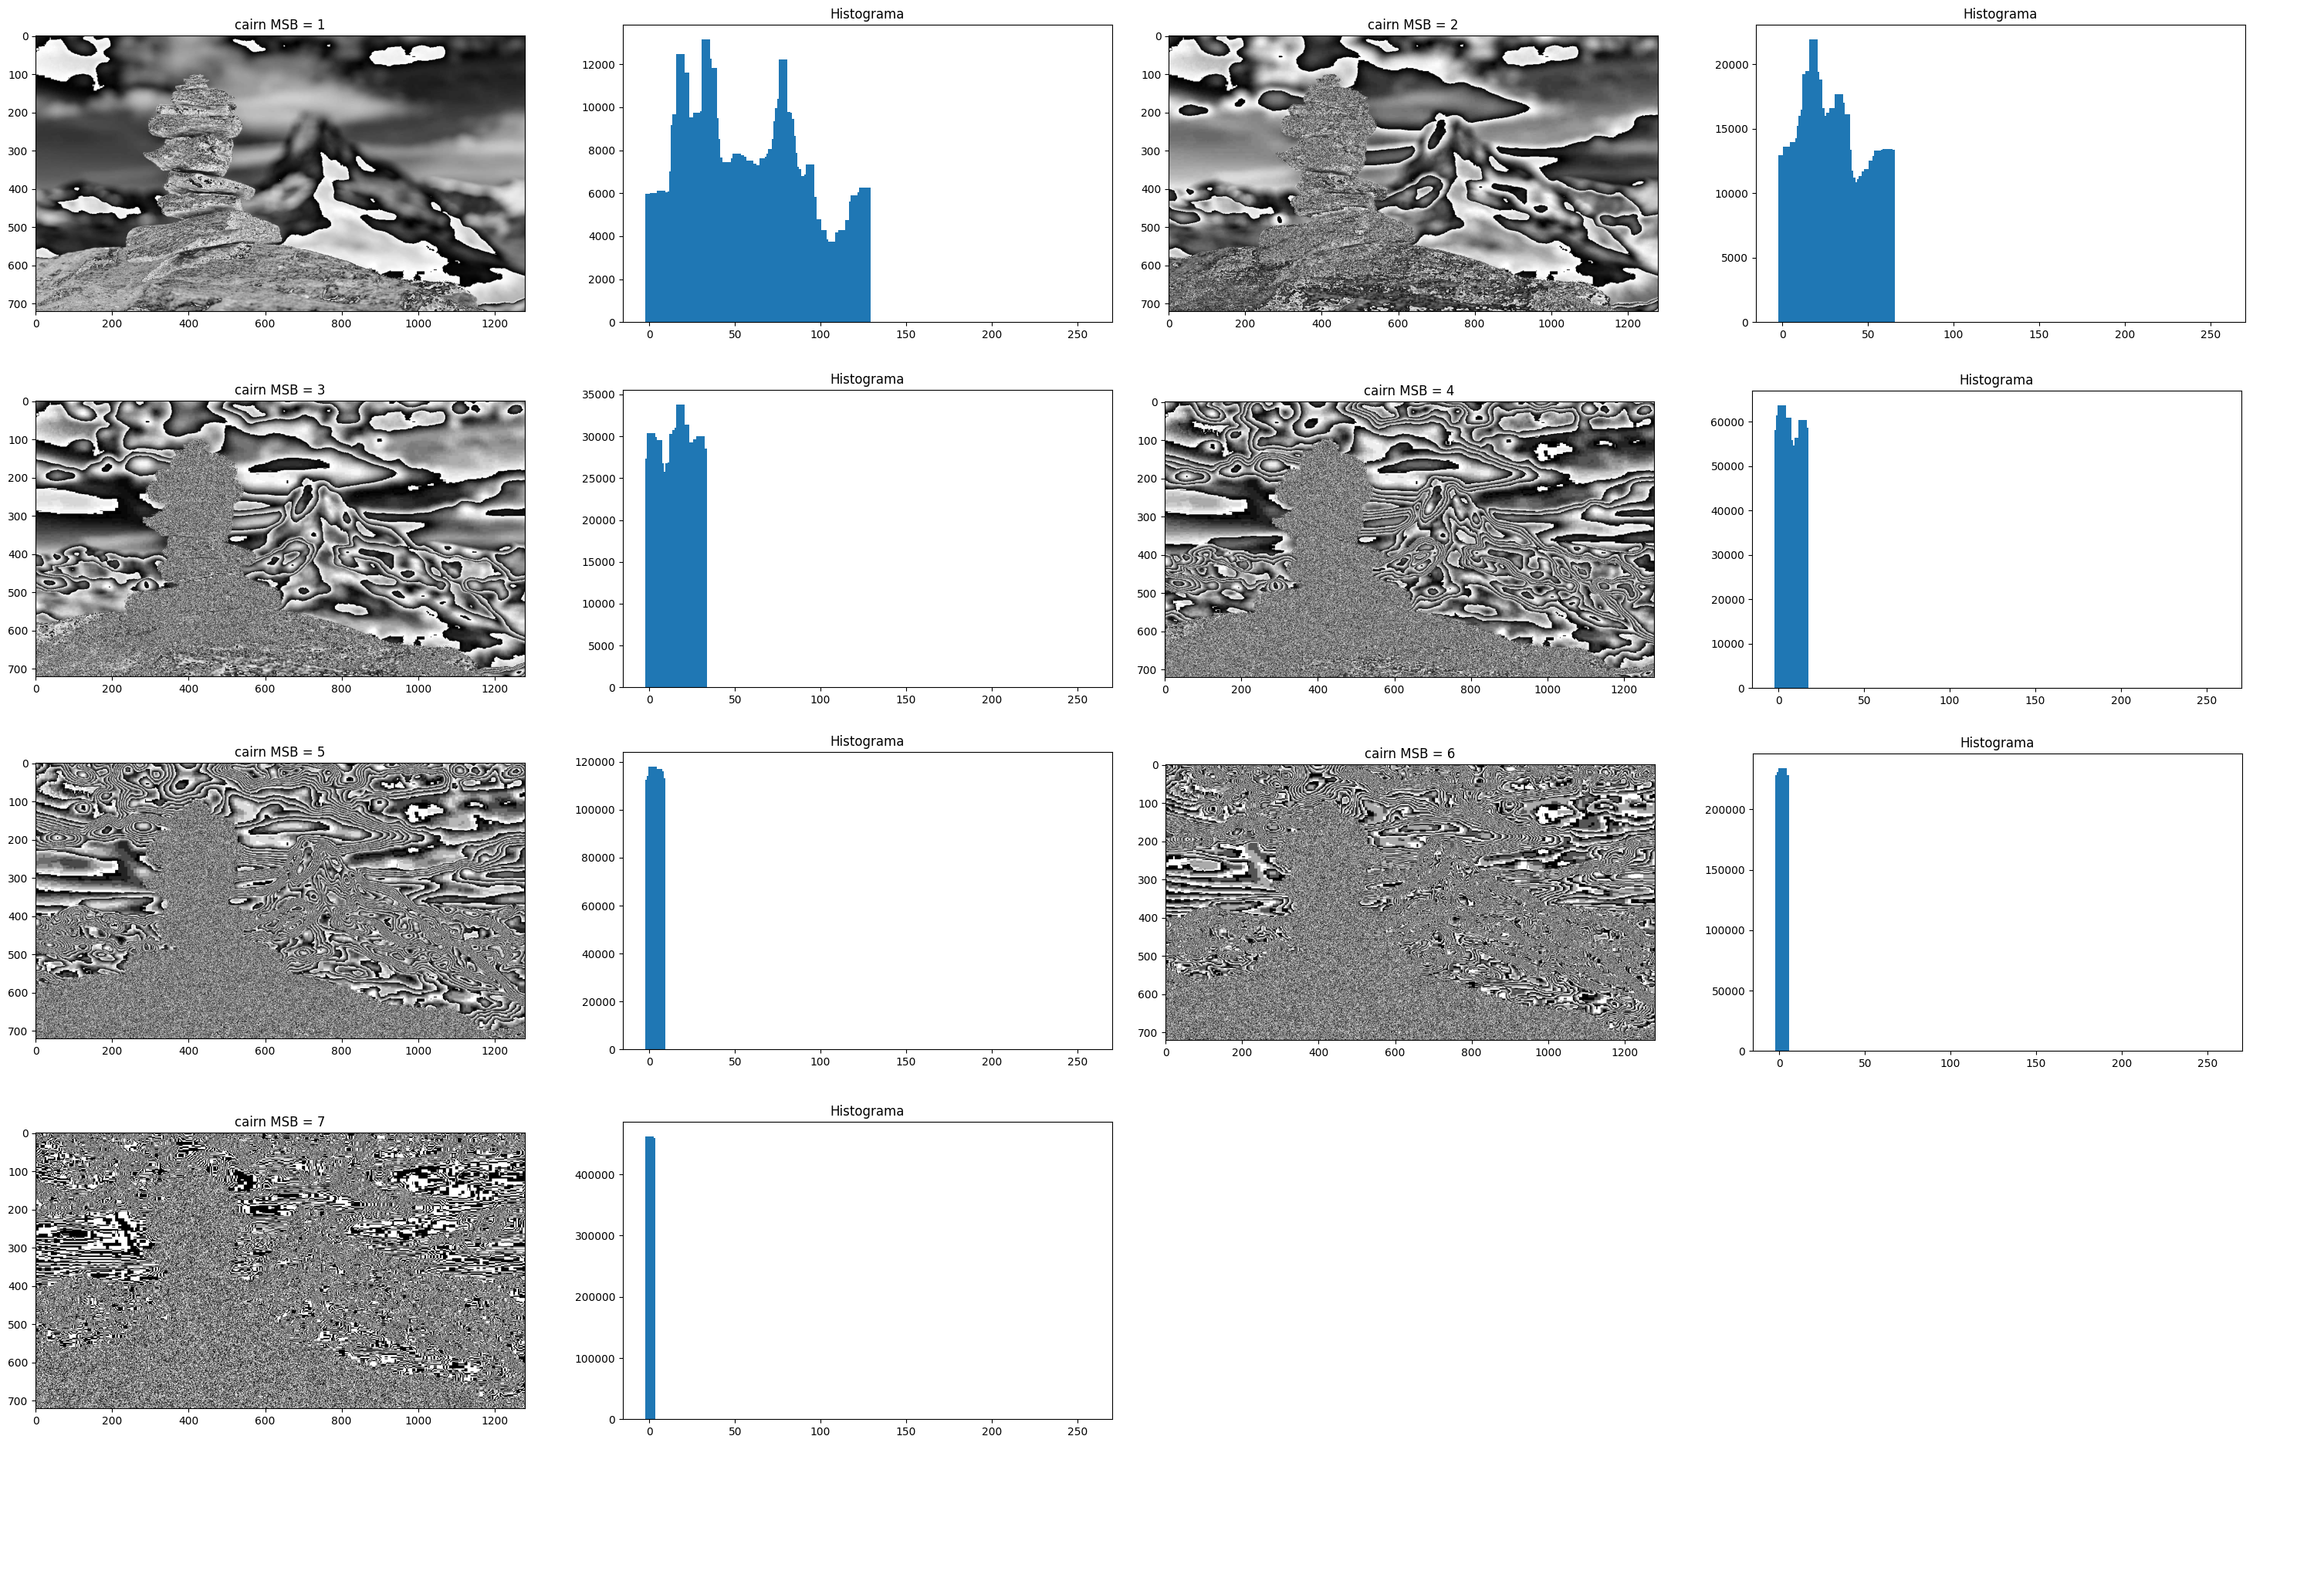
\includegraphics[width=1\linewidth]{Elementos//Figuras/cairn_msb.png}
        \caption{Da esquerda para a direita e de cima para baixo temos: Imagem Cairn com 1, 2, 3, 4, 5, 6 e 7 MSBs zerados.}
    \label{fig:cairn-msb}
\end{figure}

Percebe-se que a quantidade de ruídos apresentada é muito maior mesmo quando apenas um MSB é zerado. Isso ocorre porque, diferentemente dos LSBs, os MSBs têm grande influência sobre a informação. Dessa forma, quando o \textit{bit} mais significativo de um \textit{pixel} foi zerado, a quantidade de tonalidades possíveis para aquele \textit{pixel}, caiu pela metade.

\subsection{Análise das métricas objetivas das imagens com LSBs e MSBs zerados}

A Tabela \ref{tab:resultados-psnr-ssim} permite, por meio das métricas objetivas PSNR e SSIM, a análise da quantidade máxima de LSBs e MSBs que podem ser utilizados para ocultar informações em cada imagem. Todas as imagens que utilizaram até quatro LSBs apresentaram um SSIM acima de $0.9$, o que indica um nível alto de semelhança com a imagem original.

\begin{table}
\begin{tabular}{ccccccccc}
\hline
& \multicolumn{2}{c}{cairn} & \multicolumn{2}{c}{runner} & \multicolumn{2}{c}{shutters} & \multicolumn{2}{c}{swan} \\
& PSNR & SSIM & PSNR & SSIM & PSNR & SSIM & PSNR & SSIM \\
\hline
LSB 1 & 51.1575 & 0.9974 & 51.1388 & 0.9971 & 51.1370 & 0.9997 & 57.3143 & 0.9985 \\
LSB 2 & 42.6962 & 0.9881 & 42.7157 & 0.9862 & 42.6864 & 0.9985 & 49.3048 & 0.9943 \\
LSB 3 & 35.6999 & 0.9601 & 35.7731 & 0.9508 & 35.6897 & 0.9935 & 42.6692 & 0.9811 \\
LSB 4 & 29.3002 & 0.9016 & 28.6152 & 0.9076 & 29.2425 & 0.9745 & 36.6770 & 0.9489 \\
LSB 5 & 22.9212 & 0.8368 & 21.1971 & 0.7985 & 23.0121 & 0.9097 & 30.9843 & 0.8891 \\
LSB 6 & 17.2683 & 0.7523 & 18.8059 & 0.7843 & 17.0194 & 0.7504 & 25.9452 & 0.8202 \\
LSB 7 & 11.5796 & 0.5277 & 9.4766 & 0.5577 & 11.0111 & 0.3688 & 22.6162 & 0.7695 \\
\hline
MSB 1 & 6.9259 & 0.4390 & 7.1952 & 0.6076 & 8.2724 & 0.2938 & 28.5954 & 0.9780 \\
MSB 2 & 5.2902 & 0.2337 & 3.8795 & 0.2474 & 6.1461 & 0.0507 & 24.5492 & 0.9166 \\
MSB 3 & 4.5613 & 0.1089 & 3.5696 & 0.1169 & 5.2922 & 0.0205 & 22.8298 & 0.8587 \\
MSB 4 & 4.1211 & 0.0347 & 2.9918 & 0.0351 & 4.8618 & 0.0030 & 21.9574 & 0.8102 \\
MSB 5 & 3.9201 & 0.0099 & 2.7581 & 0.0037 & 4.6506 & 0.0003 & 21.5006 & 0.7812 \\
MSB 6 & 3.8171 & 0.0018 & 2.6761 & 0.0007 & 4.5456 & 0.0000 & 21.2674 & 0.7628 \\
MSB 7 & 3.7659 & 0.0001 & 2.6324 & 0.0000 & 4.4935 & 0.0000 & 21.1479 & 0.7510 \\
\hline
\end{tabular}
\caption{Tabela com as métricas PSNR e SSIM após modificação de \textit{bits} menos e mais significativos}
\label{tab:resultados-psnr-ssim}
\end{table}

Somente a imagem \textit{swan} com 1 e 2 MSBs (Figura \ref{fig:swan-msb}) presentou um SSIM acima $0.9$ quando os MSBs foram zerados. Isso ocorre devido ao fato de que a imagem \textit{swan} original é rica em tons escuros. Os tons escuros são representados por valores próximos a zero, o que faz com que o \textit{bit} mais significativo dos \textit{pixels} mais escuros já seja zero.
\chapter[Conclusões]{Conclusões}

Notou-se que nas regiões com predominância de tons mais escuros, a alteração dos MSBs para zero causa poucos ruídos. Já nas regiões mais claras, o ato de zerar os MSBs causa distorções muito perceptíveis, a depender da quantidade de MSBs zerados e das tonalidades predominantes naquela região. 

Por meio da análise do SSIM das imagens modificadas, percebeu-se que um número maior de LSBs puderam ser zerados sem grandes consequências nas imagens que apresentam um maior valor de informação espacial, como é o caso das imagens \textit{shutters} e \textit{cairn}. Este comportamento não ocorreu ao utilizar os MSBs.

\begin{figure}
    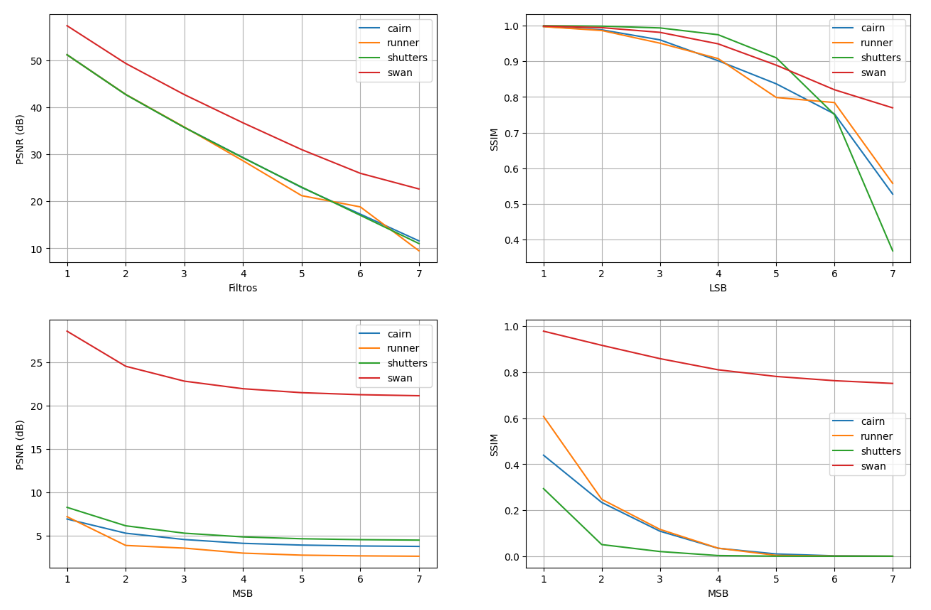
\includegraphics[width=1\linewidth]{Elementos/Figuras/graficos_lsb_msb.png}
    \caption{Gráficos de PSNR e SSIM das imagens com LSBs e MSBs zerados.}
\end{figure}




% ---
% ELEMENTOS PÓS-TEXTUAIS
% ---


% ---


\postextual
\bibliography{Elementos/references}
 
\appendix
\chapter{Apêndice A}



\chapter{Apêndice B}





\end{document}
